%
% This document is linked to this live document on Google Docs: https://docs.google.com/document/d/1MIugIo-yvuw3GTvjx8h8Qk9oVH1Pai3nUd9Qef2GzF0
% Here the April R&D tables can be found https://docs.google.com/document/d/1xrHMmOjJ_z7K5YZ4Hdz_1DQGv8P65jG1KSUfXLuqjqI
% Here the May version https://docs.google.com/document/d/1O5qI0jEeFJZT3Bu_EDPGYai72o03tiNCwENlCld0i68/edit

\documentclass{cmspaper}
\usepackage[utf8]{inputenc}

\usepackage{caption}
\usepackage{subcaption}

\usepackage{hyperref}
\hypersetup{pdfborder=0 0 0} % added to get rid of the red boxes on the TOC

\usepackage{xcolor}

% tables
\usepackage{lscape} 
\usepackage{adjustbox}
\usepackage{array}
\usepackage{booktabs}
\usepackage{multirow}
\usepackage{colortbl}

\usepackage[nomargin,inline,marginclue,draft]{fixme}
\usepackage[sorting=none]{biblatex}
\addbibresource{bibliography.bib} %Imports bibliography file

\usepackage{pgfgantt}

\usepackage{graphicx}
\graphicspath{ {./Figures/} }

% from https://design-guidelines.web.cern.ch/guidelines/ppt-colours
\definecolor{myblue}{RGB}{0,51,160} % Pantone 286C
\definecolor{myorange}{RGB}{225,94,50}
\definecolor{mycyan}{RGB}{97,197,211}
\colorlet{tableheader}{myblue!60}
\colorlet{tablerowheader}{myblue!20}
\newcommand{\trh}{\cellcolor{tablerowheader}}
\colorlet{tablerowhighlight}{myblue!5}
\newcommand{\trl}{\cellcolor{tablerowhighlight}}

%\usepackage{lineno}
%\linenumbers

\newcounter{magicrownumbers}
\preto\tabular{\setcounter{magicrownumbers}{0}}
%\newcommand\rownumber{\stepcounter{magicrownumbers}\arabic{magicrownumbers}}
\newcommand\rownumber{\refstepcounter{magicrownumbers}\arabic{magicrownumbers}}

\newcommand{\B}[1]{\textbf{#1}}
\newcommand{\UP}[1]{\multirow{-2}{*}{\B{#1}}}

\usepackage[placement=left,angle=90,color=black!40,scale=4,hshift=22,vshift=52]{background}\backgroundsetup{contents={CMS Private - Please do not share}}

\begin{document}

\newcolumntype{R}[2]{%
    >{\adjustbox{angle=#1,lap=\width-(#2)}\bgroup}%
    l%
    <{\egroup}%
}
\newcommand*\rot{\multicolumn{1}{R{90}{1em}}}

\begin{titlepage}

% select one of the following and type in the proper number:
\cmsnote{2021/XXX}

\date{29 September 2021}
\title{CMS Phase-2 Computing Model:\\ Update Document}
\begin{Authlist}
CMS Offline Software and Computing
\end{Authlist}
\vspace{0.1cm}

% >> PDF Metadata
% Do not comment out the following hypersetup lines (metadata). They will disappear in NODRAFT mode and are needed by CDS.
% Also: make sure that the values of the metadata items are sensible and are in plain text with the possible exception of the PDFtitle for a PAS. Then you can use pure TeX symbols as if on a typewriter. Examples: $\sqrt{s}=13\TeV$ => $sqrt{s}=$ 13 TeV; 32\fbinv => 32 fb$^{-1}$
% No unescaped comment % characters.
% No curly braces {} except for TeX in the PDFtitle.
\hypersetup{%
pdftitle={CMS Phase-2 Computing Model: Update Document},%
pdfsubject={CMS},%
pdfkeywords={CMS, Offline, Computing, Software, HL-LHC, Phase-2}} % limit six total


\begin{abstract}

% Recommendation
% ALL-3 Many of the potential gains depend (partly or entirely) on projects external and/or collaborative projects (eg DOMA and Event Generator/Detector Simulation improvements). In some of these cases, there is a responsibility for ATLAS and CMS to provide input/requirements; to deploy and test; and to possibly adapt the computing model to incorporate. However, in all these areas, ATLAS and CMS will need to understand the expected benefits, current status, and level of risk contributed to their overall strategy

The Phase-2 upgrade of CMS, coupled with the projected performance of the HL-LHC, shows great promise in terms of discovery potential. However, the increased granularity of the CMS detector and the higher complexity of the collision events generated by the accelerator pose challenges in the areas of data acquisition, processing, simulation, and analysis. These challenges cannot be solved solely by increments in the computing resources available to CMS, but must be accompanied by major improvements of the computing model and computing software tools, as well as data processing software and common software tools. In this document we present aspects of our roadmap for those improvements, focusing on the plans to reduce storage and CPU needs as well as take advantage of heterogeneous platforms, such as the ones equipped with GPUs, and High Performance Computing Centers. We describe the most prominent research and development activities being carried out in the experiment, demonstrating their potential effectiveness in either mitigating risks or quantitatively reducing computing resource needs on the road to the HL-LHC.

\end{abstract}

% This is a disclaimer introduced in case the document is circulated before being published to non-CMS members, such as reviewers
\vspace{0.5cm}

% \fbox{\parbox{\textwidth}{
% \B{
% \begin{center}
% \vspace{-3mm}
% DISCLAIMER
% \end{center}
% This is a draft version of the CMS-specific documentation targeting the LHCC Common Software Review scheduled for November 2021. As such, it is an internal CMS document that cannot be shared outside of the Collaboration without explicit authorization. 
% \vspace{1mm}
% }
% }
% }

\end{titlepage}

%%%%%%%%%%%%%%%%%%%%%%%%%%%%%%%%%%%%%%%%%%%%%%%%%%%%%%%%%%%%%%%%%%%%%%%%%%%%%%%%%%
% Recommendations not pin-pointed in the text
% NOTE: No C-RSG style recommendation naming was used (CMS-1, ALL-3...). The recommendations were distilled from the feedback received and translated in a list in this document: https://docs.google.com/document/d/1MIugIo-yvuw3GTvjx8h8Qk9oVH1Pai3nUd9Qef2GzF0
% o CMS-2: CMS noted concerns about the future of Cold Storage (Tape) and the need for R&D on how to best use Fast Storage. However, no related plans were presented. We encourage CMS to formulate a plan.
% --> We address only fast storage since we believe the disappearance of tape is a WLCG issue and a CMS strategy alone is not sufficient.
% o ALL-7 - Develop R&D roadmaps that are informed by strategy developed in the previous recommendation.
%   Previous Recommendation: Starting with the performance of the current software stack and existing computing model, produce tables showing how they expect CPU and storage requirements to be mitigated by current and future developments, within and outside of ATLAS and CMS, and assess the status and risks associated with each of these developments. These tables would then underpin a credible strategy.
%   --> We believe this is implicitly addressed. 
%%%%%%%%%%%%%%%%%%%%%%%%%%%%%%%%%%%%%%%%%%%%%%%%%%%%%%%%%%%%%%%%%%%%%%%%%%%%%%%%%%

\tableofcontents
\newpage

%%%%%%%%%%%%%%%%%%%%%%%%%%%%%%%%%%%%%%%%%%%%%%%%%%%%%%%%%%%%%%%%%%%%%%%%%%%%%%%%%%

\section{Introduction}

The success of the physics program of the Compact Muon Solenoid (CMS)~\cite{CMS_Paper_2008} experiment at the LHC~\cite{Evans_2008} critically depends on having  sufficient computing resources to process, store, and analyze collision and simulated data samples in a timely manner. This will be no less true in the HL-LHC era. Early estimates from 2017~\cite{Sexton_Kennedy_2018} and 2018~\cite{OCPublicResults} projected the resource needs to be several times greater than the project’s budget, assuming a flat funding profile. Updated versions of these estimates, incorporating developments in the computing model which resulted from several years of work, were presented during CMS’s contribution to the first round of the LHCC Computing Model Review~\cite{Software:2751565} in May 2020.

Since that time there has been significant progress in our understanding of how CMS plans to close the gaps between projected resource requirements and those achievable with flat budgets. The CMS collaboration has refined its flexible HL-LHC computing R\&D plan that focuses on reducing the resource needs while still improving the physics potential of the experiment. This report is an update on the status of these plans, taking into account the charge of the Stage 2 of the HL-LHC Computing Review~\cite{CERN-LHCC-2021-014} as well as the feedback and recommendations of the Stage 1~\cite{Boehnlein:2725487}. We also include reports on our progress on the use of HPC systems and heterogeneous architectures. This document is also a step along the way to preparing a Technical Design Report on CMS Offline Software and Computing for the HL-LHC era.
%, expected to be delivered in 202X (depending on when Run 4 starts). 
 
CMS has established a framework to coordinate various R\&D activities in the two broad areas of software and computing. Each R\&D activity is monitored with the aim to prioritize activities that could have a quantifiable impact on reducing processing or storage needs or mitigate a substantial risk. Milestones and decision points for each activity are defined and used to track progress.
 
An overall plan has been synthesized into a CMS strategy for computing, providing a ``roadmap'' for development while still encouraging innovative ideas from individual groups. In the end, the details of the CMS HL-LHC computing model and the resource requirements will depend on the success of these R\&D activities. Much of the work is being done by collaborators at CMS institutes, but some projects are resource limited. Some critical R\&D activities rely on external contributions, for example Geant4~\cite{Agostinelli}, ROOT~\cite{BRUN199781} and event generators. The CMS Offline Software and Computing management provides oversight of these efforts, while the activity coordination is performed in the individual development areas within the offline and computing, detector, and physics organizations. Since the management of work is primarily carried out within various CMS member institutes with funding from different countries, coordination is done with a collaborative and cooperative spirit. 
 
The outline of the document is as follows. Section~\ref{sec:scenarios} details the common machine parameters and scenarios as a baseline for the computing model. 
Then we briefly describe the CMS data processing tasks in section~\ref{sec:CMSDataProcessingTasks}. 
Section~\ref{sec:flexible_computing_model} is dedicated to the high level description of the computing model and the framework is outlined that is used for tracking and evaluating ongoing R\&D projects.
Our approach to reduce storage needs is then described in section~\ref{sec:storage_needs}.
A high level description of the network usage follows in section~\ref{sec:risks_from_networking}.
The strategy to reduce CPU needs is described for the generation, simulation and reconstruction data processing steps in section~\ref{sec:cpu_needs}.
In the next two sections, we provide an update on the status of utilizing heterogeneous architectures and accelerators (\ref{sec:usage_of_accelerators}) as well as computing resources in HPC centers (\ref{sec:usage_of_hpcs}).
Finally, in section~\ref{sec:plan_for_the_evo} we give an overview of the roadmap we have compiled, outlining CMS’s strategies to reduce the gaps between projected resource needs and what realistic budgets can provide in the HL-LHC era, discussing our projected needs for CPU, disk and tape.
Conclusions close the document in section~\ref{sec:conlusions}.

%%%%%%%%%%%%%%%%%%%%%%%%%%%%%%%%%%%%%%%%%%%%%%%%%%%%%%%%%%%%%%%%%%%%%%%%%%%%%%%%%%

\section{LHC and CMS running parameters and hardware cost evolution}
\label{sec:scenarios}
% Recommendation
% 2020-1 Describe progress towards establishing common LHC machine parameters (Common Recommendation 1 from the first review)
% ALL-5 - Iterate with WLCG and with the LHC Machine Group on a set (or sets?) of common and realistic parameters that are appropriate for baselining the computing models. Once agreed, these parameters should be used consistently. In addition to common machine and running parameters, these agreed parameters should include 
% - an agreed expected cost evolution of resources
% - the expected lifetime of hardware so that hardware replacement costs

Any projection of computing needs for HL-LHC critically depends on the assumptions of the future running conditions of the accelerator. Progress has been made towards establishing common baseline LHC machine parameters in conjunction with the ATLAS experiment~\cite{Aad:1129811}, the WLCG, and the LHC Machine Group through the LHC Program Coordination (LPC)~\cite{lpcc}. Critical accelerator inputs to the models of computing needs include the LHC schedule, the expected leveled instantaneous luminosity, the expected number of running days per year, and the H\"ubner factor, which includes effects from the overall machine availability and efficiency and the luminosity decay over a given fill~\cite{Bruning:1493022}. The current LHC schedule indicates a shutdown (LS3) in 2025-26, with otherwise full operational years, except in 2027 when the HL-LHC will be commissioned (see Figure~\ref{fig:lhc_perf}).
\begin{figure}[ht]
\centering
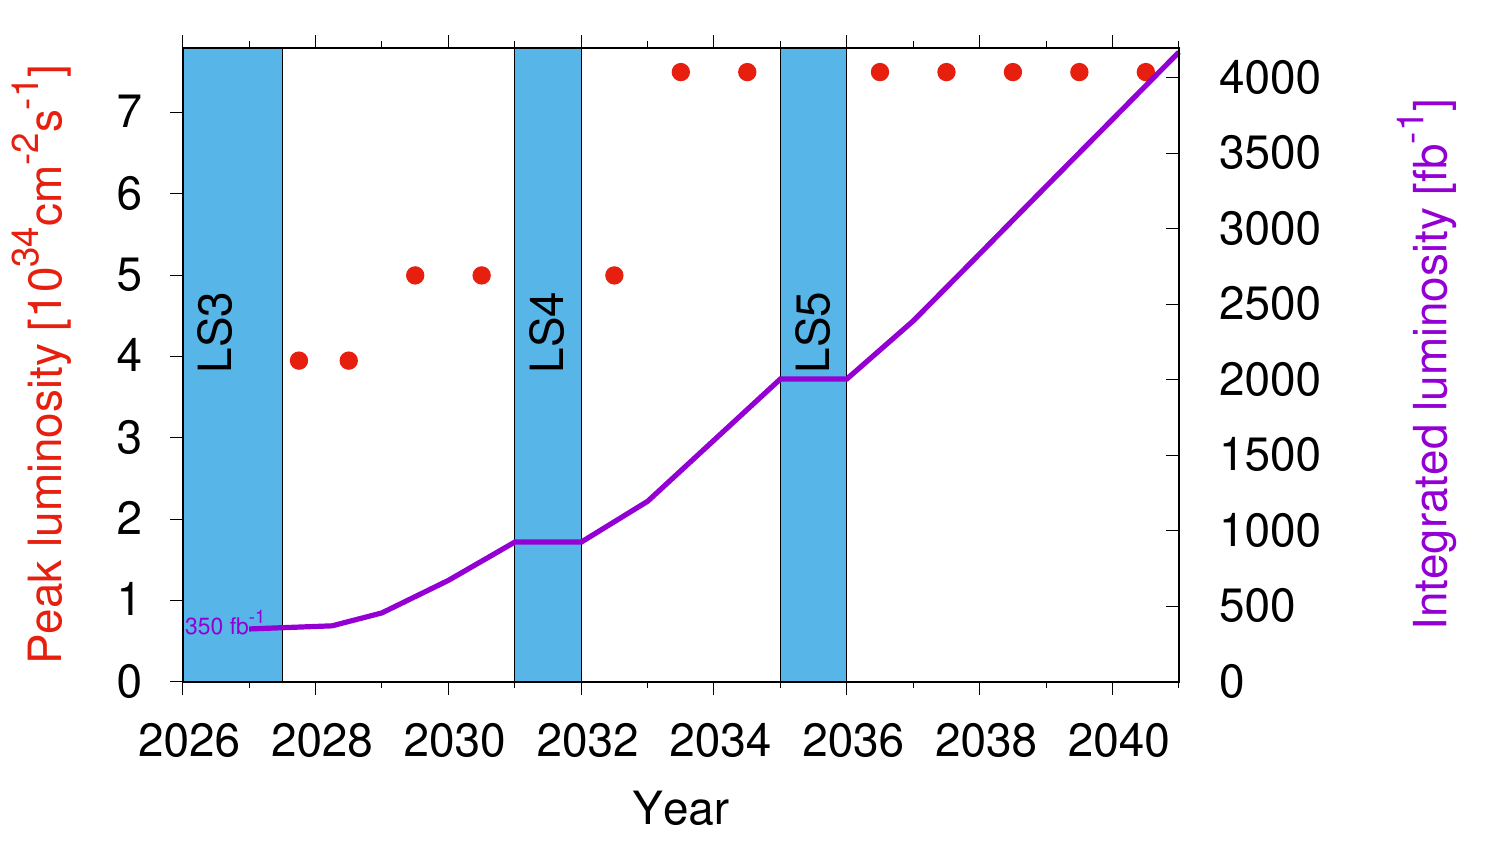
\includegraphics[trim=.1cm .1cm .1cm .5cm,clip,width=.7\textwidth]{Figures/LHC_ultimate_lumi_May_2021.png}
\caption{Forecast from~\cite{ultimate_lumi}, for peak luminosity (red dots) and integrated luminosity (violet line) in the HL-LHC era, according to the HL-LHC ultimate parameters. During Run 4, the peak pileup is 140 while, during Run 5, is 200.}
\label{fig:lhc_perf}
\end{figure}

Currently, the working scenario communicated to experiments by the LPC foresees a maximum pileup of 140 during Run 4 (instantaneous luminosity of 5 $\times$ 10$^{34}$ cm$^{-2}$s$^{-1}$) and a maximum pileup of 200 during Run 5 (instantaneous luminosity of 7.5 $\times$ 10$^{34}$ cm$^{-2}$s$^{-1}$). The top section of Table~\ref{tab:scenarios} shows the machine parameters based on the input of LPC agreed to be used for the context of this document. In addition, the yearly capacity evolution of CPU, disk, and tape resources under a flat budget agreed between the experiments and the WLCG is listed. The value for this is increased by $+15\pm5\%$, starting from a baseline of the pledged resources in 2018. This estimate includes the expected cost evolution of resources as well as hardware replacement costs. 

Experiment-specific quantities derived from these conditions, the high level trigger (HLT) rate and the numbers of collision and Monte Carlo events, are also listed in Table~\ref{tab:scenarios}. The HLT rates are taken from the CMS HLT/DAQ TDR~\cite{CMS-TDR-21-007}. The expression for the number of Monte Carlo events in billions is $9 + N\times 0.2\times L$, growing linearly with $L$, the recorded integrated luminosity in fb$^{-1}$, and is therefore not dependent on the number of events passing HLT selections. The 9 billion constant term stands for the needs of Monte Carlo events before the data taking, e.g. for commissioning or forming a trigger menu, as well as a baseline for analysis. The term $N$ represents the impact of negative weights in event generation and is equal to $1.4$ (more details about this topics can be found in section~\ref{subsec:cpu_needs_gen}). The expression is made based on experience during the previous LHC runs.

The cost of GPUs with respect to CPUs per unit of computation is estimated by CMS to be 2.8 times lower~\cite{CMS-TDR-21-007} but is not part of the common scenario. It must be emphasized that these estimates are subject to large uncertainties and represent the working scenario at the time of writing.

\begin{table}[ht]
\begin{center}
\caption{Machine parameters based on the input of LPC and common financial assumptions of budget evolution during the period 2021-2034 (top section) and CMS-specific parameters, including the CPU-GPU cost ratio per unit computation (bottom section).}
\label{tab:scenarios}
\begin{tabular}{lcc} 
\hline
\rowcolor{tableheader} \B{Parameter} & \B{Run 4 ($^\prime$27-$^\prime$30)} & \B{Run 5 ($^\prime$32-$^\prime$34)} \\
\hline  \hline
\rowcolor{tableheader} \multicolumn{3}{c}{\textit{Common}} \\ \hline
\trh LHC Energy [TeV]                             & \multicolumn{2}{c}{14}  \\
\trh  Average PU                                  & 140 & 200 \\
\trh  Integrated luminosity / year [fb$^{-1}$]    & 270 (135 in $^\prime$27) & 350 \\
\trh  Livetime pp / year [s/10$^6$]               & 6 (3 in $^\prime$27) & 8  \\
\trh  Livetime HI / year [s/10$^6$]               & 1.2 & - \\
  \hline
\trh  Yearly capacity evolution under             &  \multicolumn{2}{c}{\multirow{3}{*}{$+15\pm5\%$}} \\
\trh  flat budget for disk, CPU, and tape         &  &\\
\trh  (hardware replacement included)             &  &\\
  \hline \hline
\rowcolor{tableheader} \multicolumn{3}{c}{\textit{CMS-Specific}} \\ \hline
\trh  Prompt HLT Rate [kHz]                       & 5    & 7.5 \\
\trh  Collected events / year (10$^9$)            & 33   & 66  \\
\trh  MC events / year (10$^9$)                   & 79   & 100 \\
\hline
\trh  CPU-GPU cost ratio per unit computation     & \multicolumn{2}{c}{ 2.8x } \\
\hline
\end{tabular}
\end{center}
\end{table}

For our planning, we consider pileup 140 in Run 4 instead of 200, as previously done by CMS. However, CMS views pileup 200 as the ultimate challenge to be addressed by the software and computing tools and infrastructure. Work to meet the challenges posed by this level of pileup has already started. Some solutions discussed in section~\ref{sec:CMSDataProcessingTasks}, such as premixing of pileup samples~\cite{Lange:2015sba} for simulated events and the adoption of smaller NanoAOD data formats for analysis~\cite{Rizzi:2019rsi}, are in production and have had positive impacts already during Run 2.

Moreover, being ready to cope with the ultimate pileup before the start of Run 5 mitigates two risks. The first risk is that the LHC manages to over-achieve in terms of performance already in Run 4. The second is that during Run 4, when CMS will be a mature experiment, the necessary development effort to upgrade our software tools for pileup 200 is no longer available. For these reasons, all quantitative statements about the reduction of resource needs in the text are relative to a Run 5 production year at pileup 200, unless stated otherwise.

%%%%%%%%%%%%%%%%%%%%%%%%%%%%%%%%%%%%%%%%%%%%%%%%%%%%%%%%%%%%%%%%%%%%%%%%%%%%%%%%%%
\section{CMS data processing tasks}
\label{sec:CMSDataProcessingTasks}
CMS executes a variety of tasks on its distributed computing infrastructure for reconstructing and simulating collision data and analyzing both. CMS uses a mainly object-oriented event data model to store event information in ROOT files. Standardized groups of objects are stored in different files. Files with the same event content are described by a common data tier identifier (e.g. RAW, RECO, AOD, MiniAOD~\cite{Petrucciani:2015gjw}, NanoAOD). We expect to continue this mode of operation during the HL-LHC era.

As the first step in simulating collision data, the {\it generation} task uses Monte Carlo event generators, software packages provided by the theoretical particle physics community to generate events from theoretical principles. CMS relies on a rich set of event generators such as Pythia~\cite{Sjostrand_2006}, POWHEG~\cite{Oleari_2010}, Sherpa~\cite{Bothmann_2019} and MadGraph~\cite{Alwall:1699128}, CMS’s primary generator for matrix elements. 

The {\it simulation} task then takes the output of the generation task and models the energy deposition of particles interacting with the material in the CMS detector. Two flavors of simulation exist in two separate frameworks: Geant4-based and a parameterized fast Monte Carlo chain, also known as ``fastsim'' in CMS~\cite{Abdullin:1328345}. Geant4 has been augmented with computationally efficient techniques such as shower libraries in the forward calorimeters, specific cuts/models per particle type and detector region, and Russian Roulette~\cite{Lange_2015, Hildreth:2017vpw} for neutrons, reducing its run time.\\
The fast Monte Carlo chain is a complete Monte Carlo processing that includes a parameterized digitization and reconstruction (these steps are described below) using a simplified detector geometry~\cite{Giammanco_2014}. Datasets obtained with the fast Monte Carlo chain reproduce the output of the standard simulation and reconstruction at roughly the 10\% level approximately one order of magnitude faster~\cite{Sekmen:2242542}. Samples obtained with the fast Monte Carlo chain are usually leveraged to study systematic uncertainties or for scans in some parameter space, e.g. in the case of SUSY or other exotic signatures.

The {\it digitization} task comes next to model the electronic processing of the signal produced by the energy depositions in the detector. It also simulates the effect of additional pp interactions within the same (in-time) or neighboring (out-of-time) bunch crossings, called pileup. Historically, pileup mixing has combined a number of individual minimum-bias events with the secondary input to the digitization along with the primary simulated event. During Run 2, CMS developed and put into production the pileup ``premixing'' technique, where the combination of minimum bias events is done only once in a separate step. The digitization step in premixing mode combines a simulated primary event with a single premixed secondary event. The reading of the latter happens over the network, relying on the AAA federation~\cite{Bauerdick_2014, Bauerdick:2012st}. The premixing mode of pileup for current LHC conditions consumes less than half as much CPU time compared to the standard mode and nearly two orders of magnitude less I/O. This difference in I/O  becomes even more pronounced and unsustainable at the HL-LHC, when classical overlay of pileup minimum bias events would require the mixing of more than one thousand pileup events, including those in-time and out-of-time with the specific bunch crossing~\cite{Lange_2015}.
f
The {\it reconstruction} task executes all of the algorithms needed to interpret signals as being due to the interaction of identifiable particles with the detector. The reconstruction time per event increases superlinearly with the number of pileup events per collision due to the combinatorial nature of the most resource-intensive algorithms, such as charged-particle track reconstruction. Reconstruction output comes in several different formats designed for the different needs of the analysis tasks that follow. These formats include the RECO data tier, which is used primarily for detector component commissioning and includes full low-level detector information, the AOD (Analysis Object Data) with physics objects and their low level components. MiniAOD samples are derived from AOD datasets. The MiniAOD is an analysis format optimized for space saving thanks to techniques such as light-weight physics-object candidate representations, increasing transverse momentum thresholds for storing physics-object candidates, and reduced numerical precision when it is not required at the analysis level. NanoAOD datasets are derived from MiniAOD. The NanoAOD does not offer a persistified object oriented data model but is stored in a simple column-wise ntuple format of fundamental types and arrays thereof, containing the subset of physics quantities generally needed for analyses. 

The {\it analysis} task reduces the size of the output of the reconstruction through the filtering of events and the elimination of the information not required for a particular physics measurement. Specific event properties are calculated and information reduced to histograms or graphs, constructing a statistical interpretation of the results. Already today CMS data analysis is based on the small analysis formats, MiniAOD and NanoAOD. Also the CMS Heavy Ions community will use MiniAOD for analysis in Run 3. CMS has already produced a rich set of recipes relative to the NanoAOD tier in order to streamline the overall analysis process and plans to continue to invest in that direction.

An efficient analysis model for the HL-LHC era promises to reduce computing and storage resource needs. We foresee that the future analysis model will be based on the slimmest data format, the NanoAOD. However, at the present time it is not possible to precisely describe the future analysis model nor estimate the magnitude of the potential savings in the CPU requirements. CMS has formed an Analysis Tools Task Force to survey current methods and make recommendations for the future evolution of the analysis model. Several promising activities are also ongoing in CMS both in the areas of infrastructure~\cite{adamec2021coffeacasa}, possibly heading towards the concept of analysis facilities, and software internally in CMS, and also in collaboration with partners such as the ROOT project and IRIS-HEP~\cite{iris}.

With the increasing success of deep learning methods to tackle challenges in high energy physics~\cite{hepmllivingreview}, we are investigating and developing ML-driven applications at all levels. Before being deployed embedded within the data processing steps, models need to be trained. We call  this additional data processing step \textit{Machine Learning training}. Today, most models are basic and require a moderate amount of computing resources to be trained. However, the training of more complex models can take up to a week to converge, even using multiple GPUs~\cite{Pata:2750781}. There exist open software solutions for distributed training as well as proprietary tools~\cite{vlimant2021distributed}. Various frameworks for model optimization can be deployed on distributed resources such as HPCs or Grid resources. The usage and scale-up of such approaches is an active area of research, in case such methods and tools need to become accessible to a large number of CMS members.

%%%%%%%%%%%%%%%%%%%%%%%%%%%%%%%%%%%%%%%%%%%%%%%%%%%%%%%%%%%%%%%%%%%%%%%%%%%%%%%%%%
\section{A flexible computing model}
\label{sec:flexible_computing_model}
CMS strives to maintain a highly flexible computing model with the strategic goals of using efficiently all of the resources available to the experiment, while minimizing both hardware and personnel needs, and maximizing overall throughput. In this model, resource needs for processing, disk, archival storage, and networking capacity can be assigned to critical tasks. These goals are achieved also through trade-offs between the levels of utilization of these categories of resources, driven by their availability and cost. We aim to maintain this affordable, flexible approach to computing, primarily because substantial uncertainty exists in the market prices for hardware components used by the LHC experiments. From the memory shortage in the latter half of the previous decade to the current post-pandemic chip shortage, fluctuations in hardware prices can impact the availability of different kinds of resources. In addition, the future evolution of hardware technologies as well availability of computing resources and policies to access them must be taken into account. 

This flexible model has been working well during LHC Run 1, Run 2, and the preparation for Run 3. Traditional CPUs are being complemented more and more by accelerators, at HPCs and elsewhere. CMS has been working to improve its ability to utilize available computing power transparently, re-inventing its data processing algorithms, and orchestrating their execution on heterogeneous platforms, as discussed in section~\ref{sec:usage_of_accelerators}. National and supranational bodies are investing substantial resources in supercomputers. In the exascale era, HEP might be compelled to count on these resources for the bulk of its compute capacity. CMS has already started to take advantage of HPCs, adapting its software and computing tools to them. For example we are able to run all steps leading to Monte Carlo datasets in a chain, one after the other, on the same worker node, minimizing network usage (see section~\ref{sec:usage_of_hpcs}).

% Transition the narrative to network
Since the beginning of Run 2 and in presence of a reliable and high throughput network, the CMS computing model has been flexible enough to allow jobs to access data located at remote sites through the AAA mechanism. This feature has allowed, among other things, the incorporation of storageless sites in the distributed infrastructure. Moreover, AAA has made possible a trade-off that allowed us to reduce disk storage at the sites at the expense of a larger network bandwidth, i.e.~the premixing pileup simulation. Large datasets made of only pileup events, the so-called \textit{pileup libraries}, are now stored at CERN and Fermilab to be read remotely by simulation jobs running at Tier-1 and Tier-2 centers. 

Data caches~\cite{Fajardo_2018} can be efficiently used via remote reads. The caching approach is being actively investigated in CMS as a way potentially to reduce disk needs by hosting only the most popular data, potentially using ML-driven algorithms~\cite{aixcache, 9356236}. The Caltech and UCSD CMS Tier-2 centers already share part of their storage through a cache, called the SoCal cache~\cite{socal}.

\subsection{Tracking the progress of the computing model evolution}
\label{sec:framework}

Underpinning the strategies for the evolution of our computing model is a solid program of R\&D in the various areas of CMS Offline Software and Computing (O\&C) as well as other areas of the collaboration. Software development for the HL-LHC, in particular, is spread across the collaboration and the O\&C management works with Upgrade management to communicate priorities and track the progress. The strategic goals of CMS O\&C (discussed above in section~\ref{sec:flexible_computing_model}) are communicated regularly to our collaborators and well-understood by them, and serve as a guide to their R\&D activities. 
%CMS strives to use efficiently all of the resources (including the ever-growing fraction of HPC resources) available to the experiment, while minimizing both hardware and personnel needs, and maximizing overall throughput. 

We regularly collect information about ongoing R\&D activities in the various areas which either could have a quantifiable impact on processing or storage needs or mitigate a significant risk. In the following sections, we explore those R\&D activities which promise to reduce storage and CPU requirements in a quantifiable measure, and then consider those which facilitate our use of accelerators and HPCs. Milestones and decision points for each activity are defined and used to monitor progress. Effort needed and risks to completing the activities are also tracked. 
% The kinds of risks we consider are three, the technical risk, i.e.~the risk of R\&D program not delivering the expected computing performance improvements, the resource risk, i.e.~the risk of not having personnel with the required skills/experience to demonstrate R\&D or develop the product, and the sociological risk, i.e.~the risk of the community not reaching consensus on common solutions or organizing to deliver the product.
When there is a problem limiting an activity from progressing, the O\&C management attempts to find solutions, whether they be organizational problems, lack of sufficient effort, delays in external projects, or some other risk to sufficient progress.

%priorities
%CMS management has agreed on three main criteria for the R\&D projects to consider in case we have to implement strict prioritization, for example, if forced by a severe lack of person power. The first one is whether the reduction of computing resources can happen already during Run 3. The second one is whether the activity results in a mitigation of risks present for Run 3. The third is the ratio of potential gain weighted by probability of success/adoption and effort needed to succeed.

CMS management has agreed on three main criteria for R\&D projects to consider in cases where we would have to prioritize one over another, for example if a group had interest to work on two different lines but only the resources to choose one. The first criterion is whether the reduction of computing resources can happen already during Run 3. The second one is whether the activity results in a mitigation of risks present in Run 3. The third is the ratio of potential gain weighted by probability of success/adoption and effort needed to succeed.

Note that there are other R\&D lines which are not included in the tables of this document because they do not (yet) allow a straightforward quantitative estimation of resource savings. Still, for completeness, we describe at a high level the most promising among them in the text.
Other R\&D efforts CMS is pursuing are not reflected in the tables of this document because they bring advantages other than reduction of projected computing resource needs, e.g. reducing operational costs. One example is the containerization of the internal portfolio of computing services of CMS, such as the data discovery or workload management services, and their deployment on CERN's central Kubernetes clusters~\cite{Imran:2765040}.


%%%%%%%%%%%%%%%%%%%%%%%%%%%%%%%%%%%%%%%%%%%%%%%%%%%%%%%%%%%%%%%%%%%%%%%%%%%%%%%%%%

\section{Storage}
\label{sec:storage_needs}
HL-LHC poses a storage challenge, both in terms of disk and tape. In this section, we discuss the highlights of the planned evolution of the computing model aiming to reduce storage needs through reduction in the size of data formats, in particular the RAW data, partial prompt reconstruction, and utilization of fast storage. The descriptions of these R\&D lines, projected reductions in resource needs, milestones and decision points, and associated risks and external dependencies are summarized in Table~\ref{tab:storage_needs}.

\subsection{Data Format Size Reduction}
In the HL-LHC era, the size of the overall dataset is dominated by RAW events, the largest format permanently recorded on storage (see Table~\ref{tab:event_size}).

\begin{table}[ht]
\begin{center}
\caption{Projected event sizes for pileup levels of 140 and 200 of different tiers, compressed.}
\label{tab:event_size}
\begin{tabular}{lrr} 
\hline
\rowcolor{tableheader}           & \multicolumn{2}{c}{\B{Event size [MB]}}\\
\rowcolor{tableheader} \UP{Tier} & \B{200 PU} & \B{140 PU} \\
\hline
\hline
\trh RAW     &  5.9  & 4.3    \\
\trh AOD     &    2  & 1.4    \\
\trh MiniAOD &  0.25 & 0.18   \\
\trh NanoAOD & 0.004 & 0.004  \\
\hline
\end{tabular}
\end{center}
\end{table}

While the preparation of the new detector advances towards the Run 4, we are working with the experts of individual subdetectors to improve our understanding of the projected RAW event size with the goal of minimizing it. Up to now, detectors did not study yet the average offline RAW event size in Run 4 and Run 5, but rather focused on the dimensioning of the DAQ infrastructure. For this reason, the current RAW event sizes, shown in Table~\ref{tab:raw_size}, have to be considered as upper limits.
\begin{table}[ht]
\begin{center}
\caption{RAW event size for the individual CMS detectors~\cite{CMS-TDR-21-007}, for pileup 140 and 200. A reduction of 30\% from RAW data compression is assumed, based on Run 2 experience as well as Run 3 and HL-LHC simulations. RAW event size for offline is to be further reduced before the start of Run 4 as a result of better understanding of the new detectors, for example, HGCAL~\cite{CERN-LHCC-2017-023}. For reference, the projected RAW event size at 200 pileup considered in 2020 was 6.5~MB.}
\label{tab:raw_size}
\begin{tabular}{lrr} 
% HLT TDR: https://cds.cern.ch/record/2759072
\hline
\rowcolor{tableheader}               & \multicolumn{2}{c}{\B{Offline RAW event size [MB]}}\\
\rowcolor{tableheader} \UP{Detector} & \B{200 PU} & \B{140 PU} \\
\hline \hline
\trh Inner tracker (Pixel)           & 1.44 & 1.01  \\
\trh Outer tracker (Strip)           & 1.16 & 0.81  \\
\trh MTD                             & 0.68 & 0.48  \\
\trh ECAL Barrel                     & 0.60 & 0.42  \\
\trh HCAL                            & 0.33 & 0.33  \\
\trh HGCAL                           & 3.20 & 2.25  \\
\trh Muon system                     & 0.75 & 0.53  \\ %rounded
\trh L1 trigger                      & 0.26 & 0.26  \\ \hline\hline
\trh Total uncompressed              & 8.42 & 6.09  \\ \hline
\trh Total compressed (30\% reduction) & 5.90 & 4.26  \\
\hline
\end{tabular}
\end{center}
\end{table}

If the RAW event size needs to be further reduced with respect to the levels in Table~\ref{tab:raw_size}, a semi-processed version of the RAW format can be used, referred as to RAW$^\prime$. This approach is at the moment targeted specifically to the tracker information~\cite{CERN-LHCC-2017-009}. This technique targets heavy ions data processing already during Run 3. At the HLT, the tracker clusters are produced, the barycenter and size are calculated, and only those values are stored in the RAW$^\prime$ events instead of the full RAW event. This technique has not been put yet in production for proton-proton collisions and requires studies of potential non-trivial effects. A careful validation of the final physics output will have to be carried out inspired by the one done for the heavy ion data. This approach shows great promise, with a reduction of up to about 15\% of the whole RAW event, which potentially could be achieved for proton-proton collisions in the HL-LHC era (cf. Table~\ref{tab:storage_needs}, row 1). 

ROOT is the software technology chosen for the persistency of event data. The evolution of the present ROOT columnar format, \textit{TTree}, into the new \textit{RNtuple} aims to combine improved compression algorithms with a more compression-friendly data layout. Initial tests by the ROOT team hint to a potential size reduction of 20\% for columnar datasets featuring at least several tens of columns holding collections, e.g. properties of certain particles such as electrons or muons. The usage of \textit{RNtuple} will have a negligible effect on the size of RAW datasets, given the way in which RAW data is stored, i.e.~in a single column where a single object is streamed per row (cf. Table~\ref{tab:storage_needs}, row 2).
Reductions in the CPU cost of I/O are also expected by the targeted use of CPU-lightweight compression algorithms for often-read columns or for columns where the compression factor does not suffer much from faster compression~\cite{Blomer:2715450}. However, we believe it is early to provide a quantitative estimate of such gains. 
CMS is already working, in collaboration with the ROOT team, to integrate the existing \textit{RNtuple} with CMSSW with the aim to write NanoAOD datasets directly in the new format~\cite{maxOrok}. Such integration work will have to be extended in the future once more data formats can be handled by the new columnar storage. 

The largest possible adoption of slim data analysis formats, MiniAOD and NanoAOD, is a strategy to reduce storage needs already during Run 3 and a requirement for the successful analysis of data in the HL-LHC era. The objective of CMS is to have half of the analyses adopting NanoAOD at the end of Run 3, with the other half relying on MiniAOD, or for a very limited number of exceptions on aggressively skimmed AOD or perhaps RECO samples. The migration of analyses to NanoAOD began already at the end of Run 2. This activity does not require additional R\&D and is already quite advanced. The percentage of analyses which have adopted NanoAOD is currently 30\%. We will consider in the rest of this document, which focuses on Run 4 and Run 5, the objective of having 50\% of the analyses relying on NanoAOD as having been achieved by the end of Run 3.

\subsection{Partial prompt reconstruction}
\label{sec:partial_prompt}
% Recommendation:
% CMS-1 Parking data was outlined as a possible mechanism to enable CMS to balance the overall cost of resources needed at the Tier-0. The documents were inconsistent on how and when data parking would be used and we encourage CMS to clarify this point.

CMS has demonstrated several times since Run~1 that more data can be acquired than can be reconstructed promptly at the Tier-0~\cite{Franzoni:2016cym}. Part of the data input to offline was processed within 48 hours at the Tier-0 via the so-called prompt reconstruction, while the rest was copied to tape, or ``parked'', for later processing. The data parking campaign of 2018 led to recording and reconstructing 10 billion unbiased b-flavored meson decays~\cite{Bainbridge:2730111} which otherwise would have been impossible to collect.

During Run 1 and Run 2, all events promptly reconstructed at the Tier-0 were re-reconstructed at the end of the year when much improved calibrations were available. The idea behind partial prompt reconstruction, which is an evolution of the data parking concept, is to reconstruct promptly at the Tier-0 only a small fraction of the events recorded, parking the rest on tape to then (re-)reconstruct all events at the end of the year~\cite{Software:2751565}. Partial prompt reconstruction, therefore, would allow us to save the tape that would be used for AOD and other derived data produced promptly. It would also allow to reduce the needed computing capacity, since the majority of the data events are processed only once.

With partial prompt reconstruction, the fraction of promptly reconstructed data is reduced to an amount which is just enough to ensure data quality and the preparation of analyses. The rest of the data is transferred as usual to the Tier-0 and Tier-1 sites for the custodial copies. At the end of the LHC Run for the given year the usual reprocessing is launched on all parked and previously promptly reconstructed RAW data using all computing resources available, the processed datasets becoming available by January-February, too late for the winter conferences, but well in time for the summer ones. This limitation can be mitigated if Tier-1s are free in the first part of data taking to process a larger fraction of prompt and somehow partially recover Run 1-2-3 capabilities~\cite{Hufnagel_2015}. Likewise, if an analysis is on the critical path and needed by the winter conferences with full statistics, all of its trigger streams could be processed promptly.

This approach is not the preferred one by CMS to meet the HL-LHC computing resources requirements, although it gives us the flexibility to reconfigure the data taking chain if forced to fit in a certain budget, depending on the success of our efforts to reduce storage and computing needs. We consider this strategy an ``emergency brake''. If this this approach is adopted, it can save a significant CPU (estimated to be 30\% during a typical Run 4 year and 35\% during a typical Run 5 year), and results in modest reductions in disk and tape storage needs (10\% and 5\% respectively).

\begin{table}[ht]
{\footnotesize
\begin{center}
\caption{Impact of R\&D activities on storage requirements. All lines are expected to be completed before Run 4 or sooner, and have no impact on the ability to use HPCs or accelerators. Adoption of NanoAOD also mitigates a risk that we will have insufficient resources to analyze all of the data. Effort needed in this and subsequent tables is expressed in full-time equivalents (FTE) and may be spread out over several years or people.}
\label{tab:storage_needs}
\begin{tabular}{llllll} 
\hline

\rowcolor{tableheader} &                  &             & \B{Effort} & \B{Milestones (M) and Decision}  & \B{Risks and External} \\
\rowcolor{tableheader} & \UP{Description} & \UP{Impact} & \B{(FTE)} & \B{Points (D) (year:description)} & \B{Dependencies}       \\
\hline\hline
%%%%%%%%%%%%%%%%%%%%%
\trh \rownumber 
      & \trh RAW$^\prime$: basic processing & -15\% RAW    & 0.5 & '22 M: reduction of HI raw event size & Physics performance not \\
\trh  & \trh of RAW data from               & event size   &     & '22 D: pp physics performance & adequate after size \\
\trh  & \trh  hthe tracker                    &              & 0.5 & '23 M: reduction of pp raw event size & reduction \\ 
\hline
%%%%%%%%%%%%%%%%%%%%%
\trh \rownumber 
\trh  & \trh ROOT evolution:        & -20\% columnar &     & Migration to RNTuple:      & ROOT team cannot \\
\trh  & \trh integration of         & dataset size   & 0.5 & '23 M: Mini and NanoAOD    & deliver on time the \\
\trh  & \trh efficient parallel I/O &                & 1.5 & '24 M: Full persistent EDM & new I/O due to lack \\
\trh  & \trh                        &                &     & '26 D: switch to RNTuple   & of available effort. \\
\hline
%%%%%%%%%%%%%%%%%%%%%
\trh \rownumber 
\trh  & \trh Partial Prompt & -5\% tape  & 0.2 & '18 M: 10B b decays recorded          & Delays of physics \\
\trh  & \trh Reconstruction & -10\% disk & 0.1 & '22 M: B parking at 3kHz              & time to publication \\
\trh  & \trh                & overall    & 0.1 & '23-'25 M: Exercise parking           & \\
\trh  & \trh                &            &     & campaigns and associated              & \\
\trh  & \trh                &            &     & tape recall exercises                 & \\
\trh  & \trh                &            &     & '32 D: ``Emergency brake''            & \\
\end{tabular}
\end{center}
}
\end{table}

\subsection{Utilization of fast storage}
\label{subsec:fast_storage}
% Recommendation:
% CMS-2 CMS noted concerns about the future of Cold Storage (Tape) and the need for R&D on how to best use Fast Storage. However, no related plans were presented. We encourage CMS to formulate a plan. 
% from CMSNote-2021-001 "[...] for fast storage such as Solid State Drives, CMS needs to sustain an R&D effort to understand how to take advantage of those technologies to speedup its processing and analysis workflows. [...]"

Fast storage, such as Solid State Drives (SSD) or NVMe, represent a different Quality of Service in the storage sector. Currently, CMS does not require low latency storage as part of its pledge. However, thanks to the flexibility of the computing model, such precious resources can be already fruitfully exploited, for example in data caches at HPC centers and also in the context of high-throughput physics analysis.

%This subsection is dedicated to how CMS can take advantage of fast storage, such as Solid State Drives (SSD) or NVMe, if available to us. Currently, CMS does not require low latency storage as part of its pledge. However, thanks to the flexibility of the computing model, such precious resources can be already fruitfully exploited.

High throughput storage can be associated to data caches used to assist storage-less sites, e.g. HPCs. All CMS data processing workflows can run at HPC centers. Given the special nature of HPC resources, input datasets, e.g. for reconstruction, cannot be always placed on storage elements as if these were WLCG sites. For these cases, XRootD~\cite{xrootd2005} caches seamlessly provide the necessary input, importing data from other sites transparently upon request. Depending on the size of the allocation at the HPC center, i.e.~the number of cores at our disposal, throughput from storage can become a bottleneck. In this context fast disks are of great help. CMS successfully commissioned this solution at the INFN-CINECA Marconi machine~\cite{marconi} in 2020 to sustain the necessary I/O with a cache made of SSD drives~\cite{spiga_cache_cineca}. We plan to acquire further experience with this setup with future allocations at CINECA and elsewhere.

Fast storage enables high throughput analysis. The usage of NanoAOD is particularly important in this context as it also minimizes the CPU cost of deserialization, thanks to its simple non-object oriented layout. Table~\ref{tab:ana_rates} shows the rates achieved using a simplified version of the CMS $H\rightarrow\mu\mu$ analysis~\cite{higgstomumu}.
\begin{table}[ht]
\begin{center}
\caption{Measurements relative to a multithreaded CMS $H\rightarrow \mu \mu$ vector boson fusion analysis running on 32 CPU cores over NanoAOD input samples, compressed with LZMA, ZLIB and LZ4 algorithms~\cite{Shadura_2020}. Rates and other performance metrics are measured~\cite{dawg}.}
\label{tab:ana_rates}
\begin{tabular}{lrrrr} 
\hline
\rowcolor{tableheader} \B{Rate [kHz]}      & \B{LZMA} & \B{ZLIB} & \B{LZ4} & \B{Uncompr.} \\
\hline \hline
\trh SSD & 710 & 1121 &  1180 & 627 \\
\trh HDD &  36 &   35 &    34 &  28 \\
\hline
\end{tabular}
\end{center}
\end{table}

We plan to continue investigating the analysis throughput achievable with different storage technologies, using analysis tools such as ROOT's RDataFrame~\cite{rdataframe} and Coffea~\cite{Smith:2020pxs}. Besides an ergonomic user interface, these tools allow to transparently parallelize the execution of the analysis tasks, on a single node or on multiple nodes, therewith allowing to utilize easily the entire bandwidth between the CPUs and the storage.

%%%%%%%%%%%%%%%%%%%%%%%%%%%%%%%%%%%%%%%%%%%%%%%%%%%%%%%%%%%%%%%%%%%%%%%%%%%%%%%%%%

\section{Networking}
\label{sec:risks_from_networking}
% Recommendation
% ALL-4 - ATLAS and CMS should examine whether their future computing model overly exposes them to a risk from networking compared to other experiments.
Networking is one of the fundamental resources in the computing model of CMS, in addition to storage and computing power. When planning for the future, we are giving networking more and more equal consideration. Presently, we have no indication that CMS is exposed to risks from networking which are particularly higher than those facing other experiments. 
%However, we note that one of the main challenges ahead of us is the coming constraint on bandwidth that involves all LHC experiments operations that use the networks. Especially the shared networks in the US, Europe, Asia, Latin America and across the Atlantic and Pacific oceans. 
However, we note that one of the main uncertainties for all of the LHC experiments is the risk of bandwidth constraints in the future, especially on the shared networks in the U.S., Europe, Asia, Latin America and across the Atlantic and Pacific oceans.
Both traffic growth, cost trends for undersea networks, and the ``technology push'' of advances in switches and servers, seem to indicate that the headroom we have today may be reduced in the future.

CMS adopts measures to prevent expensive transfers and remote reads already today, for example by guaranteeing the placement of at least two replicas of the MiniAOD analysis set and pileup mixing libraries sat all times on each side of the Atlantic.
Moreover, if all investigations about data caching are successful, transfers could be further reduced to the essential ones, i.e.~the datasets or even files which are processed. 

% Old figure
% \begin{figure}[ht]
% \centering
% 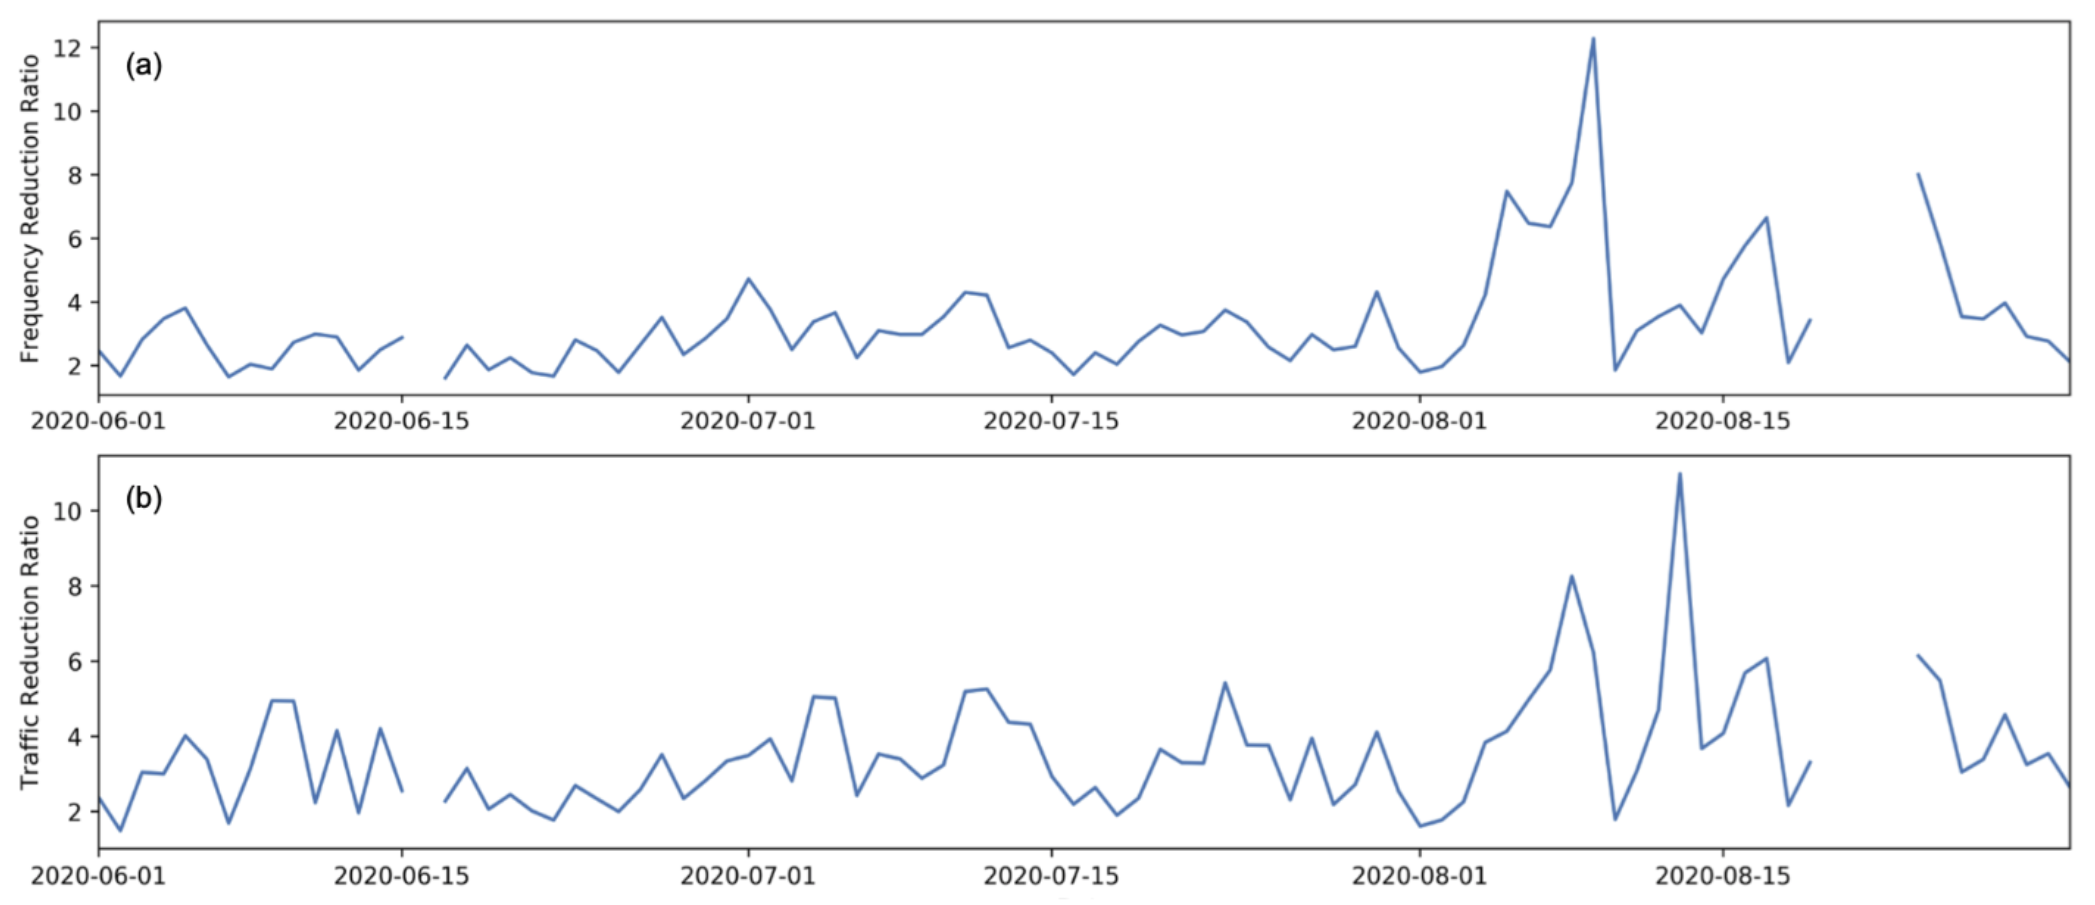
\includegraphics[width=.8\textwidth]{Figures/cachesavings.png}
% \caption{Network utilization reduction ratio in terms of (a) number of accesses and (b) volume transferred (from~\cite{inNetworkCache}).}
% \label{fig:cachesavings}
% \end{figure}

During the Long Shutdown 2 (LS2) of the LHC, significant changes took place in the computing model which reduced network usage, e.g.~the adoption of NanoAOD as the data format used for analysis, the usage of data caches, as well as the adoption of RUCIO~\cite{Rucio2019} in 2020~\cite{Vaandering:2757339}. CMS will continue to actively monitor network usage during Run 3 and put to good use its findings to further improve the flexibility of the computing model (see Figure~\ref{fig:5yotransfers}).

% New figure
\begin{figure}[ht]
\centering
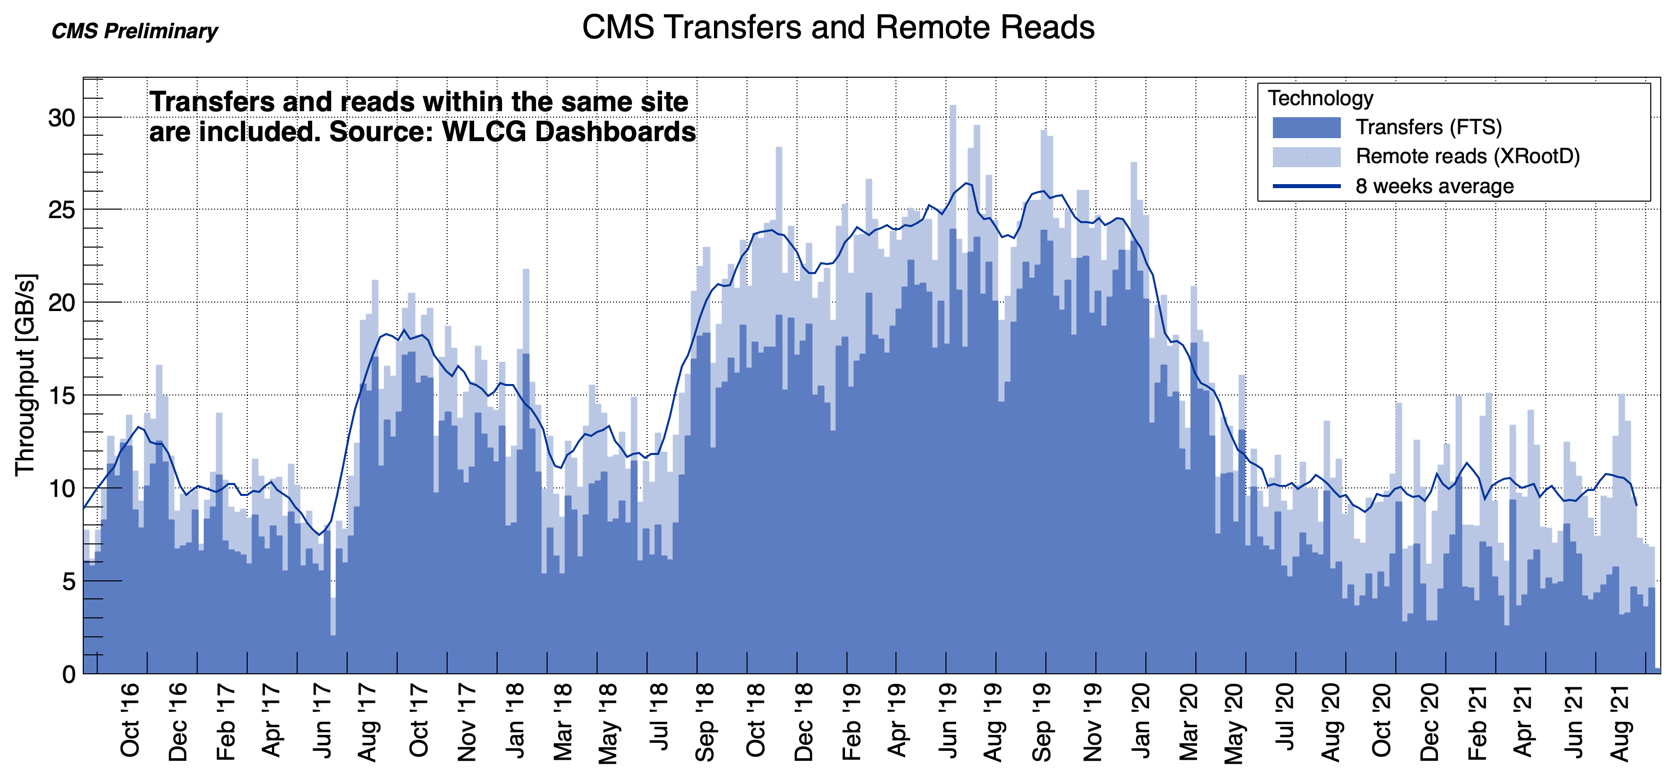
\includegraphics[width=.8\textwidth]{Figures/5yoftransfers_v2.png}
\caption{CMS transfers and remote reads during the last five years, including transfers within the same site, e.g. tape to disk at Tier-1's. The network usage is under control and needs to be closely monitored during Run 3. Data from WLCG transfer monitoring~\cite{WLCGTransfersMonitoring5y}.}
\label{fig:5yotransfers}
\end{figure}

CMS looks with interest to new projects such as SENSE/AutoGOLE~\cite{senseautogole, Monga_2020} and NOTED~\cite{noted}, new groups such as GNA-G and its Data Intensive Sciences working group~\cite{gnag}, as well as new major trends e.g.~network programmability in both switches and end systems which provide both a foundation and a good set of directions for the necessary developments for networking. There are many research and education network partners who see the opportunity to meet a challenge that will affect them as well, with the added benefits of developing systems and tools that will advance network operations with much greater programmability and manageability while supporting major science programs. We have an opportunity to start with concrete steps within FTS, RUCIO, and monitoring tools to plan to meet the networking needs for HL-LHC as new tools and capabilities are made available each year.

%All of this provides an opportunity to us to start with concrete steps involving FTS, RUCIO, and monitoring tools, and planning at the same time to meet the needs during Phase-2 with further steps matched to the capabilities and tools available each year.

%%%%%%%%%%%%%%%%%%%%%%%%%%%%%%%%%%%%%%%%%%%%%%%%%%%%%%%%%%%%%%%%%%%%%%%%%%%%%%%%%%
\section{CPU}
\label{sec:cpu_needs}
The increased granularity of the upgraded CMS detector as well as the instantaneous luminosity delivered by the HL-LHC will make the recorded events significantly more complex than the ones recorded during Run 3. Such complexity and the higher physics accuracy required in the simulation have a direct impact on the CPU needed to process and simulate the data. In this section we review the strategy of CMS to reduce the projected CPU needs for Phase-2, which focuses on the areas of event reconstruction (currently accountable for the largest share of projected CPU needs), simulation, and generation (see Table~\ref{tab:processing_times}).
\begin{table}[ht]
\begin{center}
\caption{Current processing times per event of the main steps of the CMS chain. No reduction due to R\&D work is included.}
\label{tab:processing_times}
\begin{tabular}{lccc} 
\hline
\rowcolor{tableheader}                      & \multicolumn{2}{c}{\B{Time/evt [HS06s]}}\\
\rowcolor{tableheader} \UP{Processing Step} & \B{200 PU} &  \B{140 PU} \\
\hline\hline
\trh Gen+Sim                             & \multicolumn{2}{c}{1900} \\ 
\trh Digi+PU mix+Reco                    & 5100 & 3200 \\ \hline
% Numbers from 29-6-21
% Gen 700
% Sim 1200
% DigiMix 1800/1200
% recoDQM 3300/2000
\end{tabular}
\end{center}
\end{table}

The descriptions of these corresponding R\&D lines, projected reductions in resource needs, milestones and decision points, and associated risks are summarized in Table~\ref{tab:cpu_needs}.

\subsection{Reconstruction}
% Intro, Core and CMP
Since Run 1, we have striven continuously to improve the performance of our software, guided by effective  performance monitoring tools and infrastructure embedded in the development and integration process from the earliest stages~\cite{Eulisse_2010, 4774926}.
The core libraries and tools used to build our applications and the foundation libraries they rely on are kept at the bleeding edge. This includes compilers and optimization flags, memory allocators, mathematical libraries~\cite{2025717}, and threading runtimes. In addition, we plan to continue applying incremental optimizations and modernizations to the code and algorithms, causing marginal to no impact on the final physics quality but tangible software performance increases. 
Based on experience~\cite{Reco:Chep2018} in the reconstruction code development since startup and continuing improvements of HL-LHC reconstruction software in the recent several years, 10\%-per-year speedup can be anticipated until the beginning of Run 4 (see Table~\ref{tab:cpu_needs}, row~\ref{cpu_needs:recoinc}).

With 200 pileup collisions in addition to the hard scattering, the reconstruction time per event is driven by tracking, which represents about 45\% of the total reconstruction time. The strategy of CMS to reduce tracking computing costs is twofold. The first step is the cost-guided optimization of the cut thresholds of critical quantities for tracking. Examples of such thresholds are the displacement of tracks or their transverse momentum. This kind of tuning will also benefit the reconstruction downstream, e.g. Particle Flow~\cite{Sirunyan_2017}, as well as event sizes, reducing the multiplicity of charged particles considered. The new cuts will have to be validated thoroughly and adapted in function of their impact on physics, e.g. in the B sector (see Table~\ref{tab:cpu_needs}, row~\ref{cpu_needs:ptcuts}). It should be noted that, at the time of writing, the minimum value of transverse momentum of tracks reconstructed is 200~MeV/c.
The second step is the usage of a vectorized and parallelized implementation of the combinatorial Kalman filter based track trajectory building through mkFit~\cite{Lantz_2020}. The mkFit algorithm is not in production yet but has already demonstrated promising results for Run 3 tracking. It will be integrated if verified to offer the same or increased physics quality with respect to the present solution using less CPU (see Table~\ref{tab:cpu_needs}, row~\ref{cpu_needs:mkFit}). The combined reduction of the aforementioned tracking improvements on reconstruction time can be of up to 40\%.

One of the major upgrades of the CMS Phase-2 detector is its forward calorimeter, HGCAL. This detector will offer unprecedented spatial and timing resolution. The challenge is to design fast and accurate reconstruction algorithms which can take full advantage of the information provided by the detector. Such algorithms have to scale optimally with pileup, efficiently reconstructing showers while rejecting contaminations. Presently, the HGCAL reconstruction is based on an iterative clustering framework, TICL~\cite{gouskos_loukas_2020_4088464}, and costs about 5\% of the total reconstruction time. That target will have to be kept even when more complexity is incorporated with the goal of obtaining better physics (see Table~\ref{tab:cpu_needs}, row~\ref{cpu_needs:TICL}).

It is worth mentioning that a promising set of innovative ML driven approaches to reconstruction is being investigated in CMS, even if it is too early to assess their potential impact on the reduction of projected CPU needs. A notable example is the Exa.TrkX project~\cite{exatrkx}, developing Graph Neural Network (GNN) models aimed at reconstructing particle trajectories with standards compatible with the harsh HL-LHC environment. Exa.TrkX is also exploring the scaling of distributed training of GNN models on HPC systems and the deployment of GNN models with microsecond latencies on FPGA-based real-time processing systems. 

\subsection{Simulation}
\label{subsec:cpu_needs_sim}
High-fidelity simulation, based on the Geant4 toolkit, is not the top CPU consumer in the current projections. However, simulating the Phase-2 detector takes three times longer than the current one. This is mainly due to the HGCAL geometry complexity and the need for an increased detail in the physics modeling. Compute performance has to increase while preserving or improving physics accuracy. Performance gains will come both from the evolution of the Geant4 toolkit (up to a factor of two speedup~\cite{verderi_HSF}), external to CMS, and from improvements specific to the CMS simulation application~\cite{Pedro:201921402036} in three areas. The first one is the optimization of the geometry navigation and integration of tracks in the CMS magnetic field depending on the detector region as well as energy and nature of the particle. The second is the identification of the adequate Physics List for Phase-2, based on future HGCAL test-beam analyses and recommendations of the Geant4 team. The third is the development of GFlash~\cite{Grindhammer:420530} parametrizations per particle type and per calorimeter for low-energy ranges. 
We expect the aforementioned improvements to bring a reduction of the simulation time per event of 30\%. Combining those with the evolution of Geant4, the detailed simulation of CMS could become twice as fast (cf. Table~\ref{tab:cpu_needs}, row~\ref{cpu_needs:G4inc}). 

Apart from the Geant4 based simulation and standard reconstruction, CMS can rely on the fast Monte Carlo processing chain~\cite{Sekmen:2242542}, also referred to as FastSim. This approach replaces both simulation and reconstruction to obtain Monte Carlo datasets and needs about one order of magnitude less time per event at the price of a reduced fidelity. The aspiration is to migrate a large fraction of the simulation needs to FastSim, increasing its physics quality. 
Different from the current usage of FastSim in CMS, this scenario requires substantial components of the generic background MC samples to be generated with fastsim only. This would require a much improved response modeling in FastSim relative to what is currently in use in CMS. This is under investigation.
In a scenario where all physics analysis groups would adopt a FastSim for half of the events they need the total projected compute capacity needed to obtain on average a reconstructed Monte Carlo event would be reduced by 40\%. A corollary objective is to maintain the current speed up factor over Geant4 based simulation while improving and validating physics accuracy of events. We note that a wider adoption of FastSim would serve to reduce the computing challenge by ensuring that MC requests can be fulfilled with a fast turn-around time for analysis teams (see Table~\ref{tab:cpu_needs}, row~\ref{cpu_needs:FastSim}).

\subsection{Generation}
\label{subsec:cpu_needs_gen}
% From the gen team 
The projected amount of data to be collected by the end of the HL-LHC run in the ultimate scenario is over 4~ab$^{-1}$ (see Figure~\ref{fig:lhc_perf}). Higher precision measurements will make it imperative that Monte Carlo generators provide significantly improved physics predictions, e.g. next-to-next-to-leading order (NNLO) simulations in QCD, predictions with higher jet multiplicities, and next-to-leading order (NLO) corrections in electroweak couplings. The computing cost of the generation of events, which is input to the detector simulation and reconstruction, is driven by the choice and mixture of generators used and the precision needed for particular physics analyses, e.g. NLO or NNLO. It is difficult to predict exactly the change in the mix of generators used from now until Phase-2. The baseline estimate for the per-event CPU time (see Table~\ref{tab:processing_times}) is based on an evolution of the mixture in the present Monte Carlo campaigns aimed to support Run 2 analysis. 

Recent software performance improvements in Pythia8~\cite{dimapythia82020} and Sherpa~\cite{sherpaopt2020}, which were driven from outside the Monte Carlo generators development community, and the increasing attention to the cost of event generation that led to consider traditional performance improvement techniques such as the usage of more aggressive compilation flags~\cite{valassi2021design}, indicate to us that the time per event for event generation will continue to decrease in the future. While it is difficult to predict the eventual impact on the time needed to generate an event, based on past experience it is estimated to be of the order of 10\%-20\% (see Table~\ref{tab:cpu_needs}, row~\ref{cpu_needs:geninc}). 

A crucial aspect of Monte Carlo generators for CMS is thread-friendliness, since all other data production workflows are multithreaded. In recent years CMS has upgraded its framework to be able to encapsulate thread-unsafe operations into processes rather than threads. This approach has helped maintain an acceptable level of concurrency but will not scale indefinitely. Progress by generator authors and software experts at labs and universities in the areas of thread safety and thread parallelism in Monte Carlo Generators is highly desirable.

Negative weights presently affect NLO Monte Carlo generation. The few negative weights in POWHEG are a result of small folding settings in the integration~\cite{Frixione:2007nu}. A more severe issue affects the MC@NLO approach, where negative weights are a consequence of the matching scheme of NLO MC events with a parton shower. When generating a sample, a negatively-weighted event has to be compensated by one or more positively-weighted ones. In order to obtain a correct description of the data, all these events have to be simulated, reconstructed and analyzed. Therefore, negative weights increase both the needs of compute and storage. Considering the current mixture of Monte Carlo generators foreseen by CMS for Phase-2 and the kind of physics processes needed, the impact of negative weights would translate in a 40\% increase in the number of Monte Carlo events needed for analysis.
The ultimate effect of negative weights is therefore a large uncertainty for us. However, the high attention the HEP community is paying to this problem~\cite{Frederix2020} as well as recent breakthroughs~\cite{Nason2020} reinforce the impression that this is an issue which will be solved by the time of HL-LHC (see Table~\ref{tab:cpu_needs}, row~\ref{cpu_needs:negweights}). 

\begin{table}[ht]
{\footnotesize
\begin{center}
\caption{Impact of R\&D activities on \textit{CPU} requirements. All lines except the first have no impact on the ability to use HPCs or accelerators. Note that for the Generator R\&D lines, the effort needed is divided among the various generator development groups and is largely external to CMS, as are the milestones and decision points.}
\label{tab:cpu_needs}
\begin{tabular}{llllll}
\hline
\rowcolor{tableheader} &                  &              & \B{Effort} & \B{Milestones (M) and Decision}   & \B{Risks and External} \\
\rowcolor{tableheader} & \UP{Description} & \UP{Impact}  & \B{(FTE)}  & \B{Points (D) (year:description)} & \B{Dependencies}       \\
\hline\hline
%%%%%%%%%%%%%%%%%%%%%%%%%%%%%%%%%%%%%%%%%%%%%%%%%%%%%%%%%%%%%%%%%%%%%%%%%%%%%%%%%%%%
\rowcolor{tableheader}\multicolumn{6}{c}{\textit{Reconstruction}} \\ \hline
\trh \rownumber\label{cpu_needs:recoinc}
\trh &\trh Continuous optimization & -10\%/year of    & 0.5   & '22-'27 M: Code optimizations     & \\
\trh &\trh of reconstruction code  & reco time per    &       & incl. compiler tuning and other   & \\
\trh &\trh                         & evt until Run 4  &       & core libraries e.g. math routines & \\
\hline
%%%%%%%%%%%%%%%%%%%%%
\rownumber\label{cpu_needs:ptcuts}
\trh &\trh Tracking displacement and    & -30\% of reco & 0.5 & '22-'23 M: First optimization, to be & Inability to reduce \\
\trh &\trh $p_T$ cuts cost optimization & time per evt  &     & further refined                      & timing substantially \\
\trh &\trh                              &               & 0.5 & '24-'25 D: Final tune of cuts before & and preserve physics \\
\trh &\trh                              &               &     & data taking, to be refined with data & performance\\
\hline
%%%%%%%%%%%%%%%%%%%%%
\rownumber\label{cpu_needs:mkFit}
\trh &\trh mkFit tracking tool & -10\% of reco & 2.0 & '19-'23 M: Commissioning      & Major change to critical \\
\trh &\trh                     & time per evt  & 2.0 & '24-'25 D: Replace CKF track  & component of reconstruction: \\
\trh &\trh                     &               &     & building for Phase-2          & CKF tracking implementation \\
\hline
%%%%%%%%%%%%%%%%%%%%%
\rownumber\label{cpu_needs:TICL}
\trh &\trh HGCAL reconstruction & HGCAL $<$5\%    & 2.0 & '24 M: Integrate first implementation & \\
\trh &\trh with TICL            & of reco time    & 2.0 & '25 D: Ready for production           & \\
\trh &\trh                      & per event       &     & & \\
\hline
%%%%%%%%%%%%%%%%%%%%%
\rownumber\label{cpu_needs:PPR}
\trh &\trh Partial Prompt & -35/30\% CPU & 0.2 & '18 M: 10B b decays recorded          & Delays of physics \\
\trh &\trh Reconstruction & @ 200/140 PU & 0.1 & '22 M: B parking at 3kHz              & time to publication \\
\trh &\trh                &              & 0.1 & '23-'25 M: Exercise parking campaigns & \\
\trh &\trh                &              &     & and associated tape recall exercises  & \\
\trh &\trh                &              &     & '32 D: ``Emergency brake''            & \\
%%%%%%%%%%%%%%%%%%%%%%%%%%%%%%%%%%%%%%%%%%%%%%%%%%%%%%%%%%%%%%%%%%%%%%%%%%%%%%%%%%%%
\hline \hline
\rowcolor{tableheader}\multicolumn{6}{c}{\textit{Simulation}} \\ \hline
%%%%%%%%%%%%%%%%%%%%%
\rownumber\label{cpu_needs:G4inc}
\trh &\trh Incremental improvements & -50\% of sim   & 0.5 & '22-'23 M: Investigation of techniques & Hooks and interfaces in \\
\trh &\trh in Geant4-based          & time per evt   & 0.5 & '23-'24 M: Implementation and          & Geant4 for customizing the\\
\trh &\trh simulation               &                &     & integration                            & simulation removed or limited \\
\hline
%%%%%%%%%%%%%%%%%%%%%
\rownumber\label{cpu_needs:FastSim}
\trh &\trh Faster simulation:        & 10x faster     & 2.0 & '21 M: FMC for Run 3            & Insufficient adoption of FMC \\
\trh &\trh Incremental improvements  & sim + digi +   & 3.0 & '22-'24 M: Expanded adoption,   & by analysis groups based on \\
\trh &\trh of Fast MC Chain (FMC),   & recosim        &     & re-tune for Phase-2             & inadequate physics  \\
\trh &\trh adopted by 50\% of        &                & 3.0 & '25 M: Validation, DQM, recipes & performance \\
\trh &\trh analyses                  &                &     & for corrections/systematics     &  \\
\trh &\trh                           &                &     & specific to FMC                 &  \\
\hline \hline
%%%%%%%%%%%%%%%%%%%%%%%%%%%%%%%%%%%%%%%%%%%%%%%%%%%%%%%%%%%%%%%%%%%%%%%%%%%%%%%%%%%%
\rowcolor{tableheader}\multicolumn{6}{c}{\textit{Generation}} \\ \hline
%%%%%%%%%%%%%%%%%%%%%
\rownumber\label{cpu_needs:geninc}
\trh &\trh Code performance       & -10\% of gen & $-$  & External & External generator \\
\trh &\trh improvements of MC     & time per evt &    &          & development groups \\
\trh &\trh generators used by CMS &              &    &          & \\
\hline
%%%%%%%%%%%%%%%%%%%%%
\rownumber\label{cpu_needs:negweights}
\trh &\trh Eliminate the presence    & -30\% MC evts & $-$  & External & External generator \\
\trh &\trh of negatively weighted    & for the same  &      &          & development groups \\
\trh &\trh for the samples relevant  & statistical   &      &          &  \\
\trh &\trh for CMS                   & power         &      &          &  \\
\hline
\end{tabular}
\end{center}
}
\end{table}


%%%%%%%%%%%%%%%%%%%%%%%%%%%%%%%%%%%%%%%%%%%%%%%%%%%%%%%%%%%%%%%%%%%%%%%%%%%%%%%%%%

\section{Usage of Accelerators}
\label{sec:usage_of_accelerators}

CMS strives to evolve its software to take advantage of modern architectures, including heterogeneous platforms featuring accelerators such as GPUs. Not only typical of modern HPCs, this kind of hardware is more and more commonly found at WLCG and other computing sites. CMS's interest in GPUs is based firstly on the desire to reduce the cost of computation. Secondly, we need to keep up with computer hardware technology evolution. Thirdly, as many HPC facilities have policies that their resources must be used efficiently, as required by their funding agencies, CMS must be able to take advantage of heterogeneous platforms including accelerators.

%CMS software has the capability today to run production workflows on GPUs, both on the framework side, i.e.~the capability to orchestrate the offload of work on anything external to a CPU thread, being it an accelerator or another process. 
The CMS software framework has the capability today to run production workflows on GPUs, offloading work on anything external to a CPU thread, whether an accelerator or another process. 
For Run 3, we will deploy a heterogeneous HLT farm featuring CPUs and GPUs to run the HLT reconstruction code, 30\% of which can be offloaded to GPUs. Unlike other experiments, the data processing framework as well as the detector code base is the same online and offline~\cite{Aaij:2704717}. We consider this symmetry a precious asset which we intend to preserve in the HL-LHC era.
%, unlike some other specialized solutions deployed by other experiments~\cite{Aaij:2704717}.
This sets a very solid base for CMS to grow its software stack to take advantage of accelerators at WLCG and other computing centers.

In this section we describe the activities in CMS which concern the utilization of GPUs. Those lines of activity relative to the CMSSW framework and the computing infrastructure are summarized in Table~\ref{tab:acc_fwk}, while those concerning the algorithmic aspects of simulation and reconstruction are outlined in Table~\ref{tab:gpu_sim_reco}. Unlike in the previous sections, quantitative reductions in the resources needed are not given, but rather the risks that CMS would not be able to use various aspects of heterogeneous facilities with accelerators are considered.

\subsection{Event processing framework and programming model}

Orchestrating parallel data processing work on modern and future multi-core and heterogeneous platforms requires a robust and flexible software infrastructure. The CMSSW framework, the heart of the software of CMS, orchestrates the data processing units containing the algorithms developed by domain experts in the experiment, in the areas of detector, analysis, or physics objects, for example. We will continue to invest in the development and maintenance of the CMSSW event processing framework to preserve and expand the support for multithreading, a prerequisite for offloading on accelerators, which has been in production since the beginning of Run 2~\cite{Jones_2014, Jones_2015}, up to hundreds of threads~\cite{tbuffermerge} (see Table~\ref{tab:acc_fwk}, row 1).

The CMSSW framework also allows the asynchronous and non-blocking offload of calculations to external accelerators such as GPUs, while keeping all CPU cores busy by concurrently scheduling tasks on each thread available. Offloading is possible both \textit{in-process}, i.e.~within the same process on an accelerator present on the same node, and \textit{remote}, i.e.~connecting to an external process running on the same or a separate server which is equipped with accelerators. 
The in-process offloading is the one foreseen for the start of Run 3 at the HLT to offload calculations and data to support the reconstruction algorithms written for GPUs~\cite{CMS-TDR-21-007}. The same approach can be adopted to offload machine learning inference through popular runtimes supported in CMSSW, such as the Open Neural Network Exchange ecosystem (ONNX)~\cite{onnx}. 
The remote offload has the added flexibility to be used at data centers where not all nodes are equipped with an accelerator, but can connect to servers which have them. This approach is currently being actively investigated through the SONIC technology~\cite{Duarte:2695229,Krupa_2021}. Promising results for supporting the offload of machine learning inference have been delivered, and encouraging initial tests with traditional algorithms developed for accelerators carried out (see Table~\ref{tab:acc_fwk}, row 2). It's useful to note that SONIC facilitates the execution of inference on multiple types of co-processors without changes in the client-side code in CMSSW.

Efficient exploitation of an accelerator for CMS data processing requires the mitigation of the overheads in offloading API calls as well as data transfer times from and to the device, forcing synchronization barriers detrimental to parallelism. In addition, because of the very nature of the problem to be solved, it is challenging to fully utilize efficiently a powerful GPU with the data of a single event. For these reasons, CMS is working on the evolution of data formats and algorithms for processing events in batches. 
Right now, it is difficult to assess precisely how much more throughput could be gained on top of concurrent processing of events using CUDA~\cite{10.1145/1365490.1365500} streams. The heterogeneous pixel reconstruction achieves a throughput twice as high with CUDA streams than without, so at least that level of improvement should be achievable for single algorithms with batching on platforms that do not support concurrency in kernels and memory operations. Supporting event batching in the framework would make the performance benefits available to all offloading mechanisms, reducing the dependence on platform features (see Table~\ref{tab:acc_fwk}, row 3).

Different GPU vendors provide different APIs to program their devices. CMS initially chose NVidia CUDA as the toolkit in which to write its GPU-targeted reconstruction algorithms. Developing and maintaining multiple versions of many algorithms requires significant effort and is prone to mistakes. Performance portability libraries aim to reduce those risks, providing a single-source programming model for heterogeneous computing platforms. Several options at different stages of maturity are available already, such as Alpaka~\cite{Zenker_2016}, OneAPI~\cite{oneapi, DBLP:conf/iwocl/AshbaughBBHKPSS20}, and Kokkos~\cite{CarterEdwards20143202}. 
% For the start of Run 3, CMS chose to adopt Alpaka, encapsulating as much as possible its usage to ease the future adoption of other portability layers. % https://indico.cern.ch/event/1019627/contributions/4292524/attachments/2225316/3769130/tsgOC_Apr13.pdf
Before investing heavily in any particular performance portability technology for Phase-2, CMS is understanding the strengths and limitations of the different products~\cite{Childers:2021tog}. A set of metrics has been esablished for the evaluation of the performance portability layer. These metrics include programming experience and ease of learning, performance, cost of integration into CMSSW, supported backends, maturity, and long-term prospects. Using only one portability technology within CMSSW is highly preferable to minimize maintenance effort. In order to prepare for a case that some of external libraries would use a different portability technology than in CMSSW, interoperability capabilities of the technologies are being explored as well. This work heavily depends on the evolution of the portability technologies, as well as on the evolution of the native APIs and runtimes of the different GPU vendors (see Table~\ref{tab:acc_fwk}, row 4).

\begin{table}[ht]
{\footnotesize
\begin{center}
\caption{Impact of R\&D activities in the areas of the programming model, event processing framework, and the computing infrastructure on the usage of \textit{accelerators}. Impact is characterized in terms of the mitigated risks to exploiting accelerators. Most lines are expected to be completed during Run 3.}
\label{tab:acc_fwk}
\begin{tabular}{llllll} 
\hline
\rowcolor{tableheader} &                  & \B{Impact}           & \B{Effort} & \B{Milestones (M) and Decision}  & \B{Risks and External} \\
\rowcolor{tableheader} & \UP{Description} & \B{(Risk Mitigated)} & \B{(FTE)} & \B{Points (D) (year:description)} & \B{Dependencies}       \\
\hline\hline
%%%%%%%%%%%%%%%%%%%%%%%%%%%%%%%%%%%%%%%%%%
\rowcolor{tableheader} \multicolumn{6}{c}{\textit{Data Processing Framework and Programming Model}} \\ \hline
%%%%%%%%%%%%%%%%%%%%%%%%%%%%%%%%%%%%%%%%%%
\rownumber 
\trh & \trh Development and             & Not being able to          & 3.5 & '19-'34 M: support MT platforms & I/O as bottleneck \\ 
\trh & \trh maintenance of the          & adequately use many cores  &     & efficiently at the level of     & for scaling       \\
\trh & \trh CMSSW event                 & CPUs and accelerators      &     & 100's of cores, manage offload  & (e.g. ROOT I/O)   \\ 
\trh & \trh processing framework        &                            &     & of calculation, ensure good     & \\ 
\trh & \trh                             &                            &     & functioning with evolving       & \\ 
\trh & \trh                             &                            &     & libraries.                      & \\ 
\hline
%%%%%%%%%%%%%%%%%%%%%%%%%%%%%%%%%%%%%%%%%%
\rownumber 
\trh & \trh ML inference and            & Integration of ML inference & 2.5 & '22 M: use FPGAs or other          & NVidia \\
\trh & \trh algorithm offload on        & tools in CMSSW, require     &     & co-processors, implement           & Triton \\
\trh & \trh separate process,           & computing nodes equipped    &     & (non-)ML algorithms.               & \\
\trh & \trh running on a separate       & with accelerators           &     & '22 D: Whether and how to deploy   & \\
\trh & \trh server                      &                             &     & SONIC in the Run 3 HLT, also       & \\
\trh & \trh                             &                             &     & considering data scouting          & \\
\trh & \trh                             &                             & 2.5 & '23 M: integrate inference servers & \\
\trh & \trh                             &                             &     & with workload management           & \\
\hline
%%%%%%%%%%%%%%%%%%%%%%%%%%%%%%%%%%%%%%%%%%
\rownumber 
\trh & \trh Batching event data         & Being affected by          & 1.0 & '22-'23 M: prototype batching   & \\ 
\trh & \trh in the framework            & overheads or limitations   &     & mechanisms                      & \\
\trh & \trh                             & of the achievable offload  &     & '23 D: chose batching mechanism & \\ 
\trh & \trh                             & rate due to small          & 1.0 & '24 M: start migration of       & \\ 
\trh & \trh                             & kernels or no support for  &     & framework and user code         & \\ 
\trh & \trh                             & concurrent offloads        &     &                                 & \\ 
\hline
%%%%%%%%%%%%%%%%%%%%%%%%%%%%%%%%%%%%%%%%%%
\rownumber 
\trh & \trh Performance                 & Vendor lock-in, hardware   & 2.0 & '21 M: prototypes of real CMSSW & Performance \\
\trh & \trh portability                 & price variations and       &     & algorithms using Kokkos and     & Portability \\
\trh & \trh                             & policies, not being able   &     & Alpaka                          & Libraries \\
\trh & \trh                             & to run on future           & 2.0 & '22 M: Prototype with SYCL      & \\
\trh & \trh                             & accelerators               &     & or DPC++                        & \\
\trh & \trh                             &                            & 2.0 & '23 D: Decide on a portability  & \\
\trh & \trh                             &                            &     & layer                           & \\
\hline
%%%%%%%%%%%%%%%%%%%%%%%%%%%%%%%%%%%%%%%%%%
\hline
\rowcolor{tableheader} \multicolumn{6}{c}{\textit{Computing Infrastructure}} \\ \hline
%%%%%%%%%%%%%%%%%%%%%%%%%%%%%%%%%%%%%%%%%%
\rownumber 
\trh & \trh Heterogeneous resources     & Inability to incorporate & 0.2 & '21 M: Identify simplest set of & HTCondor \\
\trh & \trh supported in the            & resources at HPCs or     &     & parameters for matchmaking,     & \\
\trh & \trh submission infrastructure   & modernized WLCG centers  &     & first HLT workflows submission  & \\
\trh & \trh                             & in the CMS pool          & 1.0 & '22-'23 M: Efficient submission & \\
\trh & \trh                             &                          &     & of reco/sim workflows as part   & \\
\trh & \trh                             &                          &     & of full processing chains       & \\
\trh & \trh                             &                          &     & within the same HTCondor pilot  & \\ 
 \hline
%%%%%%%%%%%%%%%%%%%%%%%%%%%%%%%%%%%%%%%%%%
\rownumber 
\trh & \trh Benchmarking of  & Inability to account   & 0.1 & '21 M: First version of the CMS & \\
\trh & \trh heterogeneous    & for estimate the       &     & component of the HEPScore       & \\
\trh & \trh platforms        & value of resources     &     & benchmark, that includes GPU    & \\
\trh & \trh                  &                        &     & usage (HLT sequence)            & \\
\trh & \trh                  &                        & 0.1 & '22-'23 D: Finalization of the  & \\
\trh & \trh                  &                        &     & CMS component of the HEPScore   & \\ 
\trh & \trh                  &                        &     & benchmark                       & \\ 
\hline
\end{tabular}
\end{center}
}
\end{table}

\subsection{Incorporation of accelerators in the computing infrastructure and benchmarking}

Making use of the increasingly heterogeneous and varied set of resources upon which CMS will have to rely in the HL-LHC era will require a more flexible workload management system that makes fewer assumptions about uniformity of resources as well as more automation to prevent the increase in scale and diversity of resources from generating an explosion of manual work or a reduction on the high efficiency and flexibility with which resources are currently used. 

CMS has created a Global Pool~\cite{Bockelman:2019leu} of resources, based on the HTCondor~\cite{condor-practice} and GlideinWMS~\cite{Sfiligoi:2010zz} software technologies, thanks to which we can submit jobs to all the sites available to us. Each job is described in terms of the required computing resources, such as the number of CPU cores and memory or hardware accelerator. Through a process of matchmaking, suitable resources are assigned according to the needs of each workflow. We have already expanded the resource description and job requirements used in the matchmaking of the Global Pool to include NVidia GPUs.
%, which allows basic assignment of work on resources equipped with NVidia devices, dynamically recognizing which CUDA versions and runtimes are provided by the platforms, for both production and user jobs. 
Over the next two years, we plan to acquire expertise and refine tools in order to schedule work more and more efficiently on platforms equipped with GPUs. Support for other vendors will be added, driven by the availability of their hardware for CMS use, also thanks to the advancements of performance portability in our software.
Given the anticipated evolution of CMS computational resources towards increased heterogeneity, it is not clear that a one-size-fits-all approach to decomposing workflows into data processing tasks is sustainable. A more flexible approach that supports resource-appropriate decomposition will be explored. The jobs need to be tailored for the size of the input dataset and the performance of the processing resources. This should include more flexible job splitting and merging. A possible path to achieving this could include making use the functionality of the late materialization of jobs in HTCondor (see Table~\ref{tab:acc_fwk}, row 5).

When dealing with heterogeneous resources, we consider the aspect of accounting and benchmarking to be important. This is the reason why CMS is engaged in the WLCG HEPScore Task Force~\cite{hepscoredeployment}. This group aims to identify and deploy a benchmark for computing platforms to replace HEPSpec06~\cite{hepspec06}, a tool currently used by HEP experiments to express their needs in terms of computing capacity. In the future HEPScore benchmark~\cite{HEPSCore}, real workflows from experiments will be included to assess the computing power of any given platform. CMS has already contributed an initial set of workflows, able to run on IBM POWER and ARM CPUs, including a HLT reconstruction application running for 30\% of the time on GPUs. In the next two years, and following the collegial direction taken by the task force, CMS will update and improve its contribution to the battery of benchmarks in HEPScore to help evolve the WLCG practices for estimating the compute capacity needed by experiments (see Table~\ref{tab:acc_fwk}, row 6).

\subsection{Generation, simulation and reconstruction on GPUs}
The solid architecture and robust implementation of the CMSSW framework, and its future planned developments, allow us to focus on what work can be offloaded on GPUs in the best possible way. Algorithms do not simply need to be ported, but rather re-invented to run on GPUs, taking advantage of both traditional and Machine Learning approaches. In the following we present a selection of the most prominent ongoing efforts in CMS, anticipating that most likely more will appear on the way to HL-LHC. The activities relative to the development of data processing and simulation algorithms on GPUs are summarized in Table~\ref{tab:gpu_sim_reco}.

\subsubsection{Generation}
The event generation step is orchestrated by the CMSSW framework as any other component of the data processing chain. Its peculiarity is that almost all the processing time is spent in code not owned by CMS, the event generators and the LHAPDF parton distribution functions evaluator~\cite{Buckley2015}. Depending on their design, the event generators are invoked by CMSSW as external libraries or as standalone executables encapsulated in sub-processes. In both cases, a hypothetical GPU-enabled generator could be used by CMS transparently or with a minimal integration effort. Unfortunately, at this time, no generator adopted or adoptable by CMS has the capability to leverage heterogeneous platforms even if promising efforts in this direction are ongoing~\cite{Hagiwara2013, valassivchep2021, Carrazza:2772403}. Therefore, we believe that presently it would be premature to plan for offloading any event generation on GPUs. 

\subsubsection{Simulation}
% Simulation
As discussed in section~\ref{sec:cpu_needs}, simulation is not the top consumer of computing power for CMS. However, CMS plans to offload parts of this data processing step to GPUs gradually. The initial steps will be to integrate, test, and validate in CMSSW a full simulation CMS application based on a future Geant4 version that runs efficiently on GPUs and makes effective use of HPC facilities. Its delivery is responsibility of the Geant4 team, while we are responsible for its integration in the CMS software stack. The main technical risk involved in this effort is that a Geant4 version targeted to the execution on GPUs cannot be achieved because of fundamental characteristics of the problem. However, we are confident that the integration in CMS is an achievable goal also given the previous successful experience integrating the GeantV prototype\cite{Pedro:2715335}. An accelerator-enabled version of Geant4 would allow CMS to execute about 100\% of the simulation time on GPUs (see Table~\ref{tab:gpu_sim_reco}, row 1).

Several activities based on Machine learning approaches are ongoing in the area of simulation. Even if it's early to precisely estimate their impact on projected resource needs, they show great promise.
They would also allow to use accelerators for simulation by offloading inference algorithms, embedded in the CMS fast Monte Carlo processing chain or directly in the Geant4 based application. Presently, generative techniques or other approaches such as regression or denoising are being investigated~\cite{Belayneh_2020, Erdmann_2019, butter2021ganplifying}. The work has already started by establishing a set of data, tools, and references. The next steps foresee an update of simulation frameworks to support the use of general ML algorithms. Once this is achieved, computing and physics performance results for the most promising approaches and algorithms will have to be produced to inform final decisions toward production. Any ML approach adopted widely for simulation needs to be extremely reliable, because it will be used to produce tens of billions of events per year. This poses both technical challenges, e.g. validating that reliability without actually producing that many events first, and social challenges, e.g. convincing the community of the reliability. 
Finally, even though the R\&D effort benefits from many ongoing simultaneous projects, eventually a decision will have to be made about which project(s) are put into production, with clear criteria established and agreed up in advance.

\subsubsection{Reconstruction}
% Reconstruction
Already for the beginning of Run 3 in 2022, about one third of the HLT reconstruction sequence can be offloaded on GPUs~\cite{CMS-TDR-21-007}. The same GPU algorithms, once in the context of the offline reconstruction sequence, result in an offload of the run time smaller than 5\%. However, CMS-acquired expertise in writing GPU code as well as the infrastructure for integrating, executing, and validating that code has paved the way to activities aiming to increase the percentage of offline code runable on GPUs, both dedicated to Run 3 and Phase-2 detectors, and mainly, but not exclusively, focusing on tracking. The complexity of track reconstruction algorithms increases more than linearly with pileup, making tracking one of the main consumers of compute resources in the HL-LHC environment. Quite some attention is being dedicated to the interplay of tracking algorithms and GPUs.

For Run 3 HLT processing, CMS will use a GPU-targeted pixel-only tracking algorithm~\cite{Schulte:2668183}. Work is ongoing to utilize this algorithm also offline for Phase-2 and Run 3. The success of this activity, would result in offloading to GPUs about 5\% of the reconstruction time (see Table~\ref{tab:gpu_sim_reco}, row 2).

Core part of the aforementioned pixel-only tracking is the Cellular Automaton (CA) algorithm. The CA creates a graph of interconnected doublets of hits and successively explores and prunes it to create n-tuplets of hits. We aim to extend the CA graph to make use of hits in the outer tracker, in order to build n-tuplets spanning the full silicon tracker detector. CA allows to leverage the characteristics of the Phase-2 tracker geometry to improve the algorithmic efficiency, exposing the algorithm parallelism in a way that can be exploited using GPUs or other accelerators. The success of this activity, would result in offloading to GPUs about 10\% of the reconstruction time (see Table~\ref{tab:gpu_sim_reco}, row 3).

The initial stage of the reconstruction of electrons, the seeding step, is currently accountable for 5\% of the total Phase-2 reconstruction CPU budget. An activity is presently ongoing aiming to prototype a GPU targeted Phase-2 electron seeding for Phase-2 (see Table~\ref{tab:gpu_sim_reco}, row 4). 

%HGCAL, transition from non-ML to ML
The challenges posed by the HGCAL calorimeter to event reconstruction were described in section~\ref{sec:cpu_needs}: 5\% of the total reconstruction time is accountable to this detector. Besides the aforementioned baseline, CMS is working to become able to offload it on GPUs in two ways. The first one is a adaptation of TICL and all current production components to execution on GPUs. The second one is machine learning based. The goal is also to make this new approach optimizable, and adaptable to new developments without significant maintenance burden (see Table~\ref{tab:gpu_sim_reco}, rows 5-6). 

Machine learning shows great promise and concrete results already in other parts of CMS reconstruction. Particle Flow, is currently responsible for 7\% of the time needed to reconstruct Phase-2 events. CMS is working to understand how to offload this work to GPUs, introducing the usage of graph neural networks~\cite{Pata:2750781}. If successful, this activity could be used by CMS already during Run 3, and result in an offload of about 5-7\% of the Phase-2 reconstruction sequence (see Table~\ref{tab:gpu_sim_reco}, row 7). Further use of GPU through machine learning inference could come from other reconstruction application such as calorimeter local reconstruction or jet clustering that however represent a smaller fraction of the computing budget.

\begin{table}[ht]
{\footnotesize
\begin{center}
\caption{Impact of R\&D activities in the areas of simulation and reconstruction on the usage of accelerators. Impact is quantified in terms of the percentage of CPU offloaded to GPU for certain processing steps. Most lines are expected to be completed before Run 4.}
\label{tab:gpu_sim_reco}
\begin{tabular}{llllll} 
\rowcolor{tableheader}&                  & \B{Impact}           & \B{Effort} & \B{Milestones (M) and Decision}  & \B{Risks and External} \\
\rowcolor{tableheader}& \UP{Description} & \B{(CPU Offloaded)}  & \B{(FTE)} & \B{Points (D) (year:description)} & \B{Dependencies}       \\
\hline\hline
%%%%%%%%%%%%%%%%%%%%%%%%%%%%%%%%%%%%%%%%%%
\rowcolor{tableheader} \multicolumn{6}{c}{\textit{Simulation}} \\ \hline
%%%%%%%%%%%%%%%%%%%%%%%%%%%%%%%%%%%%%%%%%%
\rownumber
\trh &\trh Integration in CMSSW        & 100\% of    & 1.0 & '23-'25 M: Prototype integration & Geant4 and related         \\
\trh &\trh of a GPU based Geant4       & sim time    &     &  of GPU Geant4 demonstrators     & R\&D activities            \\ 
\trh &\trh application                 & per evt     & 2.0 & '25-'26 M: Develop and test      & Risk: Particle transport   \\
\trh &\trh                             &             &     & workflows, e.g for HPCs          & on GPUs cannot be          \\ 
\trh &\trh                             &             & 2.0 & '26-'27 M: validation of         & achieved because of the    \\ 
\trh &\trh                             &             &     & production version               & nature of the problem      \\
\hline
% %%%%%%%%%%%%%%%%%%%%%%%%%%%%%%%%%%%%%%%%%%
% \rownumber
%   & Faster sim: ML         & 100\% of  & 6.0 & '22-'24 M: development of         & \\
%   & implementation         & sim time  &     & algorithms, testing               & \\
%   & of detector simulation & per evt   &     & comparisons among approaches      & \\
%   &                        &           & 6.0 & '24-'26 M: incorporation in CMSSW & \\
%   &                        &           &     & for large scale validation        & \\
% \hline
%%%%%%%%%%%%%%%%%%%%%%%%%%%%%%%%%%%%%%%%%%
\hline
\rowcolor{tableheader} \multicolumn{6}{c}{\textit{Reconstruction}} \\ \hline
%%%%%%%%%%%%%%%%%%%%%%%%%%%%%%%%%%%%%%%%%%
\rownumber
\trh &\trh GPU targeted pixel           & 5\% of reco       & 1.0 & '21 M: Phase-2 version for      & \\ 
\trh &\trh track reconstruction         & time per evt      &     & HLT (as per HLT TDR)            & \\ 
\trh &\trh                              &                   & 1.0 & '22 M: Exploration aiming       & \\
\trh &\trh                              &                   &     & to exploit algorithm and        & \\
\trh &\trh                              &                   &     & code in offline reconstruction. & \\
\hline
%%%%%%%%%%%%%%%%%%%%%%%%%%%%%%%%%%%%%%%%%%
\rownumber
\trh &\trh GPU targeted Cellular        & 10\% of reco      & 1.0 & '23 M: algo implemented for       & \\ 
\trh &\trh Automaton-based              & time per evt      &     & high-p$_{T}$ prompt tracks        & \\ 
\trh &\trh track building               &                   &     & '24 D: Physics performance        & \\ 
\trh &\trh                              &                   &     & acceptable @140/200 PU            & \\
\trh &\trh                              &                   & 1.0 & '25 M: algorithm can run on GPUs  & \\ 
\trh &\trh                              &                   & 1.0 & '26 M: final tuning of parameters & \\
\trh &\trh                              &                   &     & and associated validation         & \\
\hline
%%%%%%%%%%%%%%%%%%%%%%%%%%%%%%%%%%%%%%%%%%
\rownumber
\trh &\trh GPU targeted electron        & 5\% of reco       & 0.5 & '22 D: Prototype for Phase-2,     & \\ 
\trh &\trh seeding algorithm.           & time per evt      &     & then used for accurate estimation & \\
\trh &\trh                              &                   &     & of effort for the final version.  & \\
\hline
%%%%%%%%%%%%%%%%%%%%%%%%%%%%%%%%%%%%%%%%%%
\rownumber
\trh &\trh GPU targeted HGCAL           & 5\% of reco       & 2.0 & '25 M: full reconstruction,         & \\ 
\trh &\trh reconstruction with          & time per evt      &     & including high-level showers        & \\
\trh &\trh TICL                         &                   &     & implemented to run on GPU           & \\ 
\hline
%%%%%%%%%%%%%%%%%%%%%%%%%%%%%%%%%%%%%%%%%%
\rownumber
\trh &\trh HGCAL ML based               & 5\% of reco       & 5.0 & '22 M: local and PF reconstruction  & \\ 
\trh &\trh reconstruction               & time per evt      &     & model in the HGCAL region           & \\
\trh &\trh                              &                   & 5.0 & '24 M: compute time and physics     & \\
\trh &\trh                              &                   &     & performance optimized algorithm     & \\
\trh &\trh                              &                   &     & for full PF                         & \\
\trh &\trh                              &                   & 5.0 & '26 M: tune and spread knowledge    & \\
\trh &\trh                              &                   &     & about the approach to ease          & \\
\trh &\trh                              &                   &     & maintenance during data taking      & \\
\hline
%%%%%%%%%%%%%%%%%%%%%%%%%%%%%%%%%%%%%%%%%%
\rownumber
\trh &\trh GPU targeted Particle        & 5-7\% of reco     & 1.0 & '21 M: identification of the    & \\
\trh &\trh Flow also with ML            & time per evt      &     & Run 3 porting scope,            & \\
\trh &\trh techniques                   &                   &     & also considering data scouting. & \\
\trh &\trh                              &                   & 2.0 & '22 M: Phase-2 development plan & \\
\trh &\trh                              &                   &     & based on expertise acquired.    & \\ \hline
\end{tabular}
\end{center}
}
\end{table}

Table~\ref{tab:gpu_sim_reco} summarizes the projected offloading capabilities of CMS Phase-2 software. We note that offloading on GPUs does not automatically mean a reduction in needs of computing power but rather a potential reduction of costs given the more attractive price per unit of computation of GPUs with respect to GPUs (see section~\ref{sec:plan_for_the_evo}).

%%%%%%%%%%%%%%%%%%%%%%%%%%%%%%%%%%%%%%%%%%%%%%%%%%%%%%%%%%%%%%%%%%%%%%%%%%%%%%%%%%

\section{Usage of High Performance Computing Centers}
\label{sec:usage_of_hpcs}
High Performance Computing (HPC) is an asset to address scientific challenges and increase the competitiveness of industry. Substantial national and supra-national investments have been made in this area~\cite{ECP,EuroHPC} and nascent exascale machines are at the horizon. HPC machines will be part of the future scientific computing infrastructure. Being able to incorporate them in the pool of resources available to us is a strategic goal for CMS, to use efficiently all of the computing resources available to the experiment. In this section we describe the current status of the utilization of HPCs and our future plans. Note that being able to run our applications on HPCs does not reduce the projected computing needs, although it could reduce the cost per unit capacity for our funding agencies.

Today, HPCs are used in production by CMS for all kinds of central workflows, including event generation, simulation, digitization, pileup mixing, reconstruction, and creation of analysis formats MiniAOD and NanoAOD. During the past years, HPC machines contributed significantly to the processing of the Run 2 data as well as the generation of the related Monte Carlo samples. Between five and ten percent of the total used computing power dedicated to that activity came from HPCs. 
This success is also due to the flexibility of the CMS computing model and workload management system, which allows, once a worker node is available to CMS, the scheduling in sequence of all the data processing steps, keeping intermediate dataset files on the local disk without copying them to any central storage, and exporting the relevant produced datasets only at the end of the chain. Figure~\ref{fig:CoresAtHPCs} shows the scales at which CMS has been using CPU cores at various HPC facilities since the beginning of 2020.

\begin{figure}[ht]
\centering
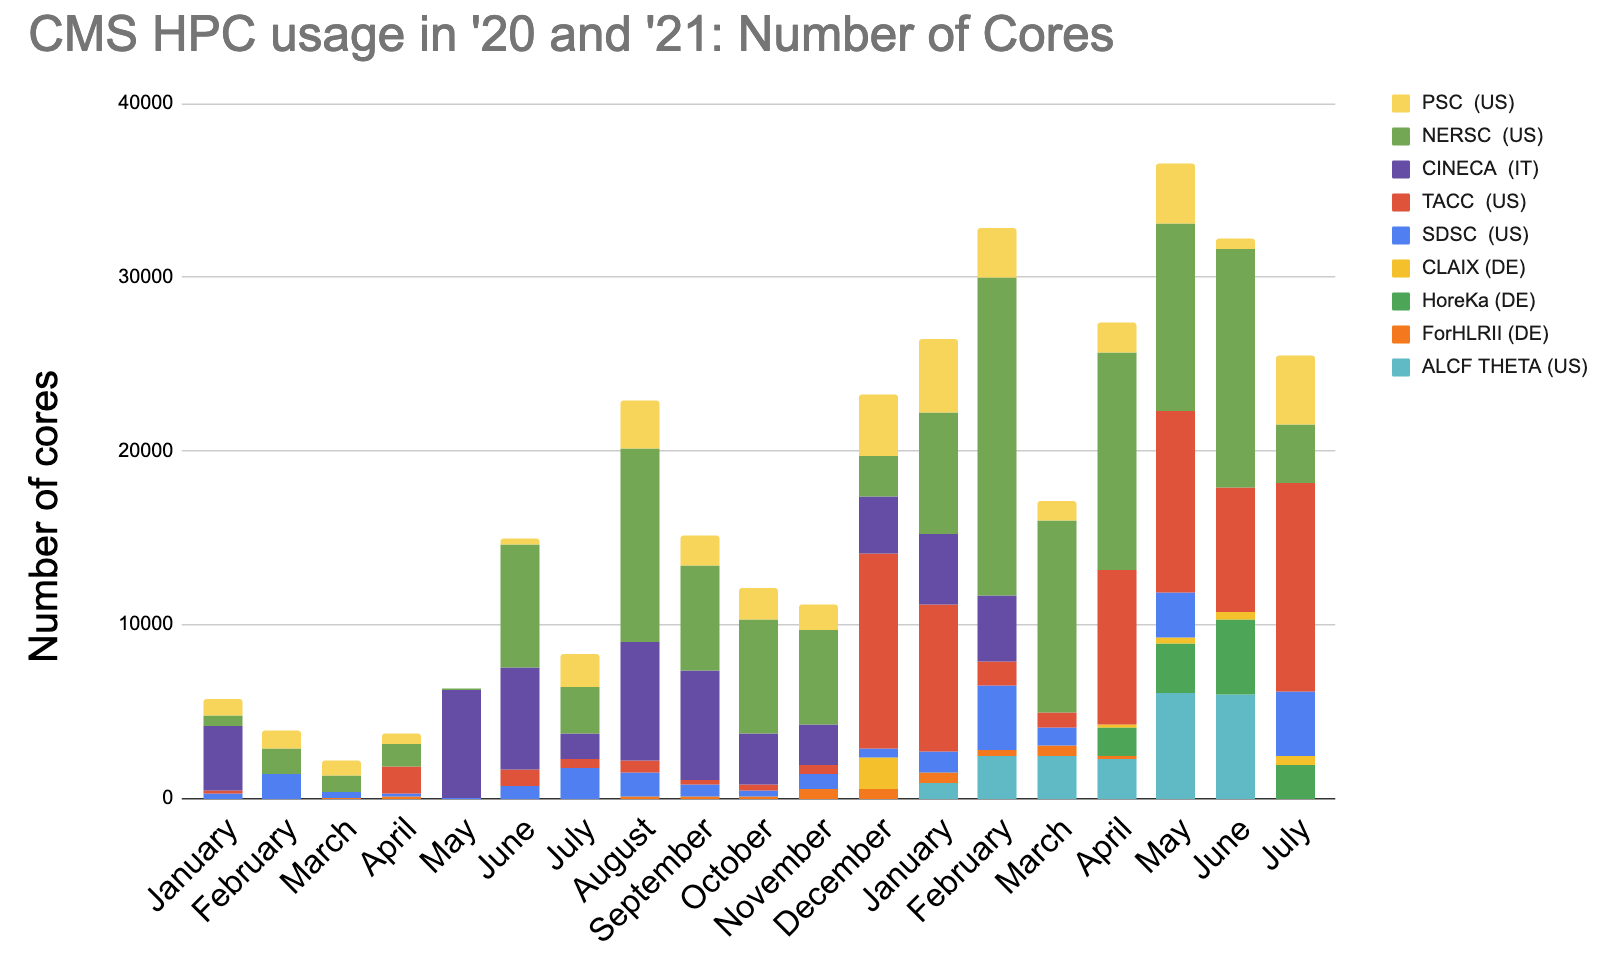
\includegraphics[width=.8\textwidth]{Figures/CoresAtHPCs.png}
\caption{Number of cores used at HPCs by CMS during the years 2020-2021. HPCs are used for all steps of central processing workflows. In 2019, the average capacity used at HPCs was of 33.6~kHS06, increasing to 108~kHS06 in 2020. The total CPU capacity pledged to CMS for those years was 2,073~kHS06. During the first seven months of 2021, the average capacity used is 307~kHS06. For comparison, the largest of the CMS Tier-1's, FNAL, pledged in 2020 260~kHS06~\cite{fnal2020cpu}.}
\label{fig:CoresAtHPCs}
\end{figure}

In the following, we review and describe the way CMS has faced and plans to face the challenges in effectively using HPCs. These are summarized in Table~\ref{tab:hpc}.

\subsection{Scalability of the submission infrastructure and the workflow managament system}
\label{sec:scalabilityWM}
The ability to fully utilize large allocations on HPCs depends on having a submission infrastructure capable of scaling up to a sufficient number of tasks and execution slots.
%One of the requirements for the incorporation of large allocations on present and future HPCs is a submission infrastructure able to manage an increasing number of workloads and large amount of resources. For CMS, this means that the capacity of the submission infrastructure, in relation to the number of execution slots in the Global Pool that can be simultaneously fed with workload, as well as the total number of simultaneously running tasks that the system can handle, has to be continuously expanded in order to satisfy the growing scales of resources available to CMS.
Working closely with the developers of HTCondor, CMS seeks to leverage innovations and new features in the software. CMS has demonstrated the ability to execute 500,000 simultaneous running jobs in 2021, a factor of 3-4 higher than current needs~\cite{globalpoolvchep2021}. We plan challenges up to 1 million simultaneous running jobs between now and 2023 (see Table~\ref{tab:hpc}, row 1).
%This can be obtained both by leveraging innovations in the software, e.g. new features in the HTCondor software, driven by the scalability needs of CMS, and expertise in their configuration. Performing internal tests, CMS has demonstrated to be able to run up to 0.5 million simultaneously running jobs in 2021, a factor 3-4 compared to current needs, as we currently execute between 100 to 150 thousand jobs concurrently~\cite{globalpoolvchep2021}. We plan more challenges in the future, culminating with a goal of 1 million jobs simultaneously managed jobs in 2023. These plans have been shared with HTCondor developers and collaboration with them is foreseen to achieve the best possible HTCondor releases for the needs of CMS (see Table~\ref{tab:hpc}, row 1). 

New HPC resources need to be integrated into CMS production. Resource availability is either relatively constant or may experience long latency from request time or short-lived peaks in capacity, as opposed to the ``constant availability'' scenario typical of traditional WLCG centers. For this reason, the workload management tools need to be able to efficiently feed a growing pool of resources, i.e.~to process requests from their initial stages on to the final scheduler queues with no sizable delays and with sufficient rate to make effective use of the available compute capacity at all times. This will require a more flexible system that makes fewer assumptions about uniformity of resources. It will also require better automation capability to prevent the increase in scale and diversity of resources from generating an explosion of manual work (see Table~\ref{tab:hpc}, row 2).

\subsection{Integration in the CMS pool of resources}

Our HPC integration strategy is based on the principle that the cost of central computing operations must not increase because of the inclusion of a new machine in the pool of available resources. For example, CMS jobs at HPCs use the same container images and the same software distribution through CVMFS~\cite{Blomer_2011} as the ones running on traditional WLCG sites. In production, three different HPC integration strategies have been adopted up to now: HEPCloud~\cite{Holzman:2291124}, site extension~\cite{Boccali:2020lcd, dellAgnello:2019tnw}, and \texttt{COBalD/TARDIS}~\cite{manuel_giffels_2018_2240606, max_fischer_2018_1887873}.

HPC resources located in the U.S., the country providing the largest computing power of all HPCs available to CMS in 2020, are integrated via HEPCloud, a gateway located at Fermilab. CMS workloads are centrally assigned to HEPCloud, as if it were a Grid site, to then run at the connected facilities. During 2020, HEPCloud allowed CMS to profit from allocations at NERSC, SDSC, PSC, and TACC HPC centers.

Italy was the second largest provider of HPC resources to CMS during 2019 and 2020 through the Marconi A2 machine at INFN-CINECA. The HPC nodes were configured as an elastic extension of the CNAF Tier-1, connected with a 40~Gbps link, and were receiving work targeted to the standard WLCG site, relying on its central storage. From the perspective of central computing operations, nothing besides an increased capacity at the Tier-1 was noticeable.

Germany, the third largest provider of HPC resources to CMS in 2020, supplied temporary resources not dedicated to WLCG. These resources, whether they are HPCs, local university clusters, or clouds, are incorporated with a HTCondor Overlay Batch System (OBS). Two instances of such OBS exist, one at the KIT Tier-1 and one at the RWTH Tier-2. Through this mechanism, additional resources are enabled to join the common HTCondor Global Pool, and CMS jobs are entitled to run on local university clusters and nearby HPCs, such as ForHLRII~\cite{forhlr2}, HoreKa~\cite{horeka} or CLAIX~\cite{claix}. The interfaces for the batch systems available on the different machines are provided by \texttt{TARDIS} tool, while load balancing happens through \texttt{COBalD} application.

Allocations at HPCs can be granted for generic CMS work or for particular types of studies, e.g. Phase-2 related workflows. Presently, these kind of resources are utilized through manual assignment of adequate workloads. CMS is gaining experience with these kinds of restricted allocations, expecting that in the future they will be more common. For those HPCs seen as extension of Tier-1s, workload assignment works as usual, and filters are enabled at the matchmaking level to ensure the suitability of the workflows. Another example is the ALCF Theta allocation in 2021 (see figure ~\ref{fig:CoresAtHPCs}), where CMS was allowed to run only jobs targeting Phase-2 studies. CMS's plan for the future foresees the development of a service to synchronize the existing tools to allow them to match available work in the queue to a particular allocation type. A substantial increase of these kinds of allocations will also have to be accompanied by an even more fluent communication among analysis groups, curators of the CMS dataset, and managers of the distributed infrastructure to ensure proper description and injection timing of dataset requests (see Table~\ref{tab:hpc}, row 3).

\subsection{Utilization of network-segregated resources}

The pilot-based late binding model of CMS~\cite{Belforte:2014iba} foresees the execution of generic, multi-core HTCondor pilots, which then connect to the central workload management to claim payload jobs. A similar mechanism will be adopted by ALICE during Run 3~\cite{Buncic:2011297, jalien1, jalien2}. This approach and the need to read non-event data such as calibrations required worker nodes to have internet connectivity until 2020~\cite{Software:2707937,Software:2707936}. That requirement represented a hurdle for some HPCs. CMS has two ways to overcome that limitation being commissioned at the time of writing.

Even if not connected to the internet, network-segregated worker nodes can typically connect to bastion or login nodes. The first solution is a modification of the standard containerized environment of CMS jobs, where all the traffic is rerouted to one or multiple edge nodes establishing a SOCKS5 tunnel~\cite{tsocksigsc}. Being a layer below the application level, this solution is future-proof with respect to changes in the protocols, services and type of connections, in contrast to specific edge services providing proxies for specific needs. The bandwidth available is limited by the tunnel endpoints. Still the connection capabilities have been proven to be sufficient to re-route management traffic (e.g. HTCondor connections) as well as the distribution of software via CVMFS and non-event data for up to three thousands cores and one single edge node. Future tests at scale with data intensive workflows will be performed if needed.

Very restrictive environments might prevent the deployment of the aforementioned tunneling solution. One such example is the BSC computer center in Spain, hosting the Mare Nostrum HPC. Thanks to a formal collaboration between the HTCondor team and CIEMAT members at the Spanish Tier-1, an edge service was prototyped that allows the replacement of the usual network communication with a shared file-system based communication path~\cite{AntonioD}. The deployed infrastructure allowed the utilization of about 10 thousand CPU cores simultaneously for real simulation workloads of CMS via a single bridge machine. Tests will be performed in the next months for utilization at scale and, if successful, integration in the CMS workload management system will take place.

\subsection{Architectures and platforms}
The hardware available at HPCs is expected to be far less uniform than on the Grid, both in terms of the presence of accelerators, the utilization of which was treated in section~\ref{sec:usage_of_accelerators}, but also the CPU architecture, which may differ from the canonical x86\_64 available on the Grid for more than a decade. From the software point of view, CMS is well prepared to run its workflows on ARM and POWER little endian architectures. The integration and unit testing of CMS code on those platforms is being performed and regular CMSSW releases targeting those architectures created~\cite{ModernizingTheCMSSoftwareStack}. The support for ARM started in 2012, while the first release targeting POWER was installed in CVMFS from 2016. Regular installations of non-x86\_64 releases on CVMFS started in May 2020.

We plan to preserve the support on ARM and POWER for which the likelihood to obtain an allocation is higher (see Table~\ref{tab:hpc}, row 4).
Thanks to an allocation on the Marconi100 machine at INFN-CINECA, CMS was recently able to carry out a technical test of its software on the POWER9 architecture running thousands of multithreaded jobs. In order to achieve this goal, the workload management tools had to be adapted for the new architecture, paving the way for an analogous test on ARM processors, if an allocation on an HPC featuring them became available. This was the first example of large statistics samples processed on non-x86 processors at LHC.

Recent and upcoming HPC installations provide a significant fraction of their compute power via GPUs. The R\&D program by CMS (see section \ref{sec:usage_of_accelerators}) aims to enhance the software to exploit those resources efficiently. The developments in the workflow management as well as the submission infrastructure layer will also efficiently target GPUs provided at HPCs. GPU usage can be expected to be a prerequisite for future HPC allocations.

\begin{table}[ht]
{\footnotesize
\begin{center}
\caption{Impact of R\&D activities on the effective usage of HPCs in the area of incorporation of resources into the CMS pools. Impact is characterized in terms of the mitigated risks to exploiting HPCs. Most lines are expected to be completed before Run 4.}
\label{tab:hpc}
\begin{tabular}{llllll} 
\rowcolor{tableheader} &                  & \B{Impact}            & \B{Effort} & \B{Milestones (M) and Decision}  & \B{Risks and External} \\
\rowcolor{tableheader} & \UP{Description} & \B{(Risks Mitigated)} & \B{(FTE)} & \B{Points (D) (year:description)} & \B{Dependencies}       \\
\hline\hline
\rownumber
\trh &\trh Submission          & Inability to accommodate and  &     & Run simultaneously & HTCondor and evolution    \\ 
\trh &\trh infrastructure      & and exploit new, substantial, &     & and efficiently:   & of its components (e.g.   \\
\trh &\trh scalability         & resources in the CMS pool.    & 0.2 & '21 M: 0.5 M jobs  & the collector service)    \\
\trh &\trh                     &                               & 0.2 & '22 M: 0.75 M jobs & not sufficiently          \\
\trh &\trh                     &                               & 0.2 & '23 M: 1.0 M jobs  & performant.               \\ 
\hline
%%%%%%%%%%%%%%%%%%%%%%%%%%%%%%%%%%%%%%%%%%
\rownumber
\trh &\trh Evolution of the    & Inability to integrate new    & 1.5 & '23 D: Cost/benefit analysis  & \\
\trh &\trh workload management & computing resources, operate  &     & for workflow description,     & \\
\trh &\trh system              & them in steady state, process &     & task decomposition, data      & \\
\trh &\trh                     & dataset requests with         &     & scheduling                    & \\
\trh &\trh                     & sufficient rate to use        & 1.0 & '24 D: Overall design.        & \\
\trh &\trh                     & available compute capacity.   & 2.0 & '26 M: Design development     & \\
\hline
%%%%%%%%%%%%%%%%%%%%%%%%%%%%%%%%%%%%%%%%%%
\rownumber
\trh &\trh Allocation aware    & Inability to leverage        & 1.0 & '22 M: requirement gathering,     & \\
\trh &\trh campaign and        & allocations characterized by &     & prototyping                       & \\
\trh &\trh production planning & constraints on the type of   & 1.0 & '23 M: Full implementation of     & \\
\trh &\trh and management      & physics in the work to       &     & functionality in a new or         & \\
\trh &\trh                     & be executed.                 &     & existing service                  & \\
\trh &\trh                     &                              & 1.0 & '24 M: Further devops activities, & \\
\trh &\trh                     &                              &     & hand over to operators            & \\
\hline
%%%%%%%%%%%%%%%%%%%%%%%%%%%%%%%%%%%%%%%%%%
\rownumber
\trh &\trh Architectures and   & Inability to use allocations  & 0.2 & '21-'34 M: Keep ARM and IBM & \\ 
\trh &\trh platforms           & on HPCs featuring non-x86\_64 &     & POWER9 integration builds   & \\
\trh &\trh                     & CPUs. Bugs undermining code   &     & working and tests passing.  & \\
\trh &\trh                     & reliability not visible on    &     & Keep all utilities and      & \\
\trh &\trh                     & x86\_64 CPUs.                 &     & scripts independent from    & \\
\trh &\trh                     &                               &     & the CPU architecture        & \\ \hline
%%%%%%%%%%%%%%%%%%%%%%%%%%%%%%%%%%%%%%%%%%
%Evolution of resource   & n/y/y & Inability to leverage HPC/Cloud &  0 & 21: Evaluate the Decision Engine    & 22: Test the scalability and  & & \\
%acquisition beyond the  &       & allocations and provision HPCs  &    & framework in a testbed environment  & continue the project only if  & & \\
%traditional Grid model  &       & in a manner consistent with     & .5 & 22: Perform scalability tests       & acceptable or a clear plan to & & \\
%                        &       & organizational business rules   & .5 & 23: Deployment in production,       & make it such can be formulated & & \\ 
%                        &       & and budget constraints.         &    & replacing glideinWMS frontend       & & & \\
%                              &               &       &       &     &                                 & & \\ 
%\hline
\end{tabular}
\end{center}
}
\end{table}

%%%%%%%%%%%%%%%%%%%%%%%%%%%%%%%%%%%%%%%%%%%%%%%%%%%%%%%%%%%%%%%%%%%%%%%%%%%%%%%%%%

\section{Plans for the evolution of the CMS Computing Model towards Phase-2}
\label{sec:plan_for_the_evo}

In the previous sections, we have given details of the various R\&D activities in CMS that aim to reduce resource needs in the HL-LHC era or which mitigate risks to and enable the efficient use of HPCs and accelerators. Tying everything together into a coherent plan for the evolution of the CMS computing model, we consider in this section each category of R\&D activities, their estimated impacts, and probability of success by a certain time, either the beginning of Run 4 or Run 5. 

For activities which reduce resource requirements or costs, the impacts are quantitative and can be multiplied by the associated probability of success to determine a risk-adjusted overall impact, to be compared to the expected evolution of computing capacity from now through Phase-2. Probabilities of success are estimated taking into consideration the associated risks to the technical completion of the R\&D, including provisioning of sufficient effort, and are grouped as ``high'', ``medium'', or ``low''. In the following, to assess the overall \textit{weighted probable impact} of R\&D lines, we assign a weight of 100\% for ``high'' probability of success or applicability, 50\% for ``medium'', and 20\% for ``low''. The \textit{optimistic impact} is calculated by simply combining the individual impacts without weights.

For HPCs, most of the activities enable the efficient utilization of the resources and are harder to quantify in terms of computing resources reductions, and are therefore classified as ``critical'', ``important'', or ``optional'' in terms of their impact on the plan. With accelerators, there are potential savings in terms of lowering CPU processing requirements, financial benefits due to relative costs, as well as policy-centered impacts since access to facilities that provide accelerators may enforce their utilization as a condition for continued use. 

From time to time new ideas for R\&D projects arise which may have additional, unforeseen impacts. It is natural, however, that as an experiment ages, effort to produce transformative advancements generally declines, underscoring the need to make progress in resource accessibility and requirement reduction as soon as possible. Such an approach also mitigates the risk of LHC performing significantly above expectations already during Run 4.

\subsection{R\&D lines which reduce projected needs of computing resources}
\label{sec:lines_which_reduce}

In Sections~\ref{sec:storage_needs} and~\ref{sec:cpu_needs}, we considered several R\&D lines which aim to reduce with a quantifiable estimate the storage or computing requirements in Phase-2. Note that many of the lines can be applied even before the start of Run 4, so we consider whether the impacts will be applicable before the start of Run 4 or Run 5.

Considering first our strategy to reduce storage requirements, one focus has been reducing the size of the RAW event in collaboration with CMS sub-detectors experts. The present RAW event size is an upper limit estimated for the DAQ design and we expect to reduce it further in the future with more and more studies carried out by the detector community, e.g. considering radiation damage. Further reductions may be possible by storing partially processed objects in the tracker information. The overall impact of this R\&D would be a 15\% reduction in the RAW data size, but the probability of applicability to proton collision data as opposed to heavy-ion we judge to be ``medium''. Turning to the other main data formats, AOD, MiniAOD, and NanoAOD, advances in the ROOT columnar storage point to a 20\% reduction in size of each of these tiers. We judge the probability of success to be ``medium''. The results of these R\&D lines are expected to be usable before the start of Run 4. The building blocks of the strategy to reduce storage needs are summarized in Table~\ref{tab:summary-storage}. 

\begin{table}[ht]
\begin{center}
\caption{Summary of impact by Run 4 of R\&D lines on the storage requirements, per data tier, and associated probabilities of success or adoption. Further details are available in section~\ref{sec:storage_needs}.}
\label{tab:summary-storage}
\begin{tabular}{lccccc} 
\hline
\rowcolor{tableheader}                                         & \multicolumn{4}{c}{\B{Impact per data tier}}      & \B{Probability} \\
\rowcolor{tableheader} \multirow{-2}{*}{\B{Short description}} & \B{RAW}    & \B{AOD}  & \B{MiniAOD} & \B{NanoAOD} & \B{of Adoption} \\
\hline \hline
\trh RAW$^\prime$                   & -15\%  &   -   &   -   &   -   & medium \\
\trh ROOT RNTuple                   &   -    & -20\% & -20\% & -20\% & medium \\ 
\hline 
\trh Optimistic impact              & \trl-15\%  & \trl-20\% & \trl-20\% & \trl-20\% &        \\
\trh Weighted probable impact       & \trl-7.5\% & \trl-10\% & \trl-10\% & \trl-10\% &        \\
\cline{1-5}
\end{tabular}
\end{center}
\end{table}

% CPU part
For R\&D activities which reduce the requirements in terms of CPU, we considered in this document three steps of the CMS workflow which are affected, usually as a percentage savings: generation, simulation, and reconstruction. The overall impact therefore depends on the relative proportions of each to the overall processing budget of the experiment in Phase-2. 

%GEN part
The event generators community is increasingly paying attention to code performance. We assume a 10\% runtime reduction overall for the Phase-2 mix of generators, judging its probability to be ``high''.

%SIM
The reduction of the projected CPU for high-fidelity simulation will be a result of CMS specific techniques and a Geant4 speedup. The CMS specific techniques are the navigation and integration of tracks carried out as a function of detector region and particle energy, the identification of the Physics List based on the future HGCAL test-beam and the development of a GFlash parametrization per particle type and calorimeter for low-energy ranges. The combined impact of the aforementioned CMS specific and Geant4 R\&D efforts would be a 50\% reduction in the time necessary for high-fidelity simulation and we judge its probability to be ``high''. 

%RECO
Reconstruction is accountable for the largest amount of projected CPU usage in the HL-LHC era. CMS will continue to improve incrementally  event reconstruction code as well as core libraries such as mathematical routines or memory allocators. We estimate the impact of this work to be of 50\% of the reconstruction time per event, with a ``medium'' probability. The most expensive step of event reconstruction is tracking of charged particles. For this step, CMS envisages two main R\&D lines. The first one is the optimization of the cuts and parameters of tracking, for example charged particles transverse momenta. The impact of this work is 30\% of the entire reconstruction sequence and we judge the probability of success to be ``high''. The adoption of the mkFit tracking tool could boost by an additional 10\% the aforementioned reconstruction speedup. We judge the adoption of mkFit to be ``high''. 

The strategies aiming to reduce CPU needs in the HL-LHC era are summarized in Table~\ref{tab:summary-cpu}. 

\begin{table}[ht]
\begin{center}
\caption{Summary of impact by Run 4 of R\&D lines on the CPU requirements, per processing step, and associated probabilities of success or adoption. Note that the overall impacts are obtained multiplicatively, since the individual contributions are uncorrelated. Further details are available in section~\ref{sec:cpu_needs}.}
\label{tab:summary-cpu}
\begin{tabular}{lcccc} 
\hline
\rowcolor{tableheader} & \multicolumn{3}{c}{\B{Impact per processing step}}                   & \B{Probability} \\
\rowcolor{tableheader} \multirow{-2}{*}{\B{Short description}} & \B{Gen} & \B{Sim} & \B{Reco} & \B{of Adoption} \\
\hline \hline
\trh Generators code performance improvements      &  -10\%  &     -  & -      & high     \\ 
\trh CMS and Geant4 improvements                   & -       & -50\%  & -      & high     \\ 
\trh Optimization of Reco code + Core libraries    & -       &     -  & -50\%* & medium   \\
\trh Tracking cuts optimization                    & -       &     -  & -30\%  & high     \\ 
\trh mkFit                                         & -       &     -  & -10\%  & high     \\ \hline
\trh Optimistic impact                             & \trl-10\%  & \trl-50\%  & \trl-70\%  &          \\  
\trh Weighted probable impact                      & \trl-10\%  & \trl-50\%  & \trl-50\%  &          \\
\cline{1-4}
\footnotesize{* -10\% year-over-year improvement until Run 4.} \\
\end{tabular}
\end{center}
\end{table}

% Improvements from changes in the way we do things: Nano, FastSim and Partial Prompt
Next we summarize three changes in the way event generation, simulation, and prompt reconstruction can be performed in Phase-2, discussing their projected impacts on CPU, disk, and tape resource needs and their probabilities of success.
%(cf. Table~\ref{tab:two_scenarios_params}).

% NanoAOD adoption
The largest adoption possible of the slimmest analysis format, NanoAOD, is a goal of CMS. In particular we want to reach the adoption of NanoAOD by 50\% of the analyses by the end of Run 3, starting from today's percentage, 30\%. Given that we are so near to the goal and no additional R\&D or integration work is needed, we consider this level of adoption in the baseline of our Phase-2 computing model.

% Negative weights
The solution of the problem of negative weights (see section~\ref{subsec:cpu_needs_gen}) can be considered a significant change %in how data processing is carried out 
because it reduces the overall usage of CPU and storage without reducing time per event or event sizes. We believe that the probability of success of this external R\&D activity is ``high''.

% Fast sim
For what concerns the fast Monte Carlo processing chain, which replaces both simulation and reconstruction, the projected gain for the CPU dedicated to obtain a Monte Carlo reconstructed event would be of 40\% if adopted for half of the events. We judge this probability to be ``low''. However, we underline the importance of the fast Monte Carlo chain to support studies such as scans of the phase-space or studies requiring fast turnaround.

% The Emergency Brake (Notbremse)
Finally, there is the approach of partial prompt reconstruction. We consider this strategy an ``emergency brake'' to be used in case other efforts to reduce the CPU requirements to fit into the expected budget evolution fail. 
The probability that we continue to use partial prompt reconstruction for special streams during Run 3 is clear, but adopting this strategy more broadly in Run 4 or Run 5 would have an impact on the efficiency of the physics program of CMS.
Such a strategy would result in CPU savings of 35\% (30\% with a pileup level of 140), mainly at the Tier-0, and also a disk and tape savings of about 10\% and 5\% respectively.

% % This table was perhaps redundant. The content is indeed included in table tab:two_scenarios_params
% \begin{table}[ht]
% \begin{center}
% \caption{Summary of impact of R\&D lines aiming to change our current operation mode. Since we consider the partial prompt reconstruction an emergency measure, we do not provide a value for its probability of adoption.}
% \label{tab:summary-approaches}
% \begin{tabular}{lcccc} 
% \hline
% & \multicolumn{3}{c}{Impact per resource type}                          & Probability of\\
% Short description                             & CPU     & Disk  & Tape  & Adoption/Success \\ \hline \hline
% Solution of the negative weights problem      & -Y\%    & -Y\%  & -Y\%  & high   \\
% Fast Monte Carlo chain for half of the events & -X\%    & -     & -     & low    \\ 
% Partial Prompt Reconstruction                 & -X\%    & -X\%  & -X\%  & -      \\ \hline
% Optimistic impact                             & -X\%    & -X\%  & -X\%  &        \\  
% Weighted probable impact                      & -X\%    & -X\%  & -X\%  &        \\
% \end{tabular}
% \end{center}
% \end{table}

\subsection{R\&D lines which enable the utilization of accelerators}

Following the successful deployment of GPUs in the Run 3 HLT, CMS aims to offload part of its offline data processing chain to accelerators, such as GPUs. Our goal is to take advantage of heterogeneous architectures, at HPCs or elsewhere, for example at future WLCG centers.

The first three elements necessary to achieve this goal are the support of heterogeneity in the data processing framework, an adequate programming model as well as an enabling computing infrastructure (cf. Table~\ref{tab:summary-gpu-fwk}).

The CMSSW framework must efficiently orchestrate calculations, offload to accelerators and I/O using order of hundred threads and remain compatible with the most recent software technologies, such as threading runtimes. We judge the impact of this activity ``critical'' and its probability of success ``high''. Since having an accelerator on the same node where the application is running might not always be possible, an R\&D line was described to obtain the flexibility necessary to leverage remote accelerators. Its impact is judged ``important'' and its probability of success ``medium''.

The processing of HEP data is traditionally event-based. However, this approach, might not be the most efficient when data and kernels have to be communicated between host and device, especially if mechanisms analogous to CUDA streams are not supported by the accelerator. Batching events together in the CMSSW framework mitigates the performance penalties linked to the treatment of individual events. The impact of this R\&D line is ``important'' and we assessed its probability of success ``high''. The experiment-specific code base should be only one and usable for CPUs and accelerators. In order to achieve this goal, a good performance portability layer has to be identified. We judge the impact of this R\&D line to be ``important'' and its probability of success to be ``high''.
Accelerators and their capabilities have to be visible to the workload management system through the submission infrastructure in order to make happen the best possible matching between resources available and type of work to be done. The activities ongoing in CMS to support accelerators in the submission infrastructure have a ``critical'' impact and their probability of success is judged to be ``high''. Finally, a contribution to the WLCG HEPScore Working Group was described which aims to benchmark heterogeneous platforms with real CMS applications. For CMS, benchmarking of heterogeneous platforms has an ``important'' impact and, given the status of the current benchmark, we believe the probability of success is ``high''.

\begin{table}[ht]
\begin{center}
\caption{Summary of impact of R\&D lines on the utilization of GPUs and associated probabilities of success or adoption. Further details are available in section~\ref{sec:usage_of_accelerators}.}
\label{tab:summary-gpu-fwk}
\begin{tabular}{lccccc} 
\hline 
\rowcolor{tableheader}                                         &                              & \B{Probability}  \\
\rowcolor{tableheader} \multirow{-2}{*}{\B{Short description}} & \multirow{-2}{*}{\B{Impact}} & \B{of Success}   \\
\hline \hline
\trh Development and maintenance of CMSSW                  & critical  & high      \\
\trh ML and algorithm offload on separate process          & important & medium    \\
\trh Batching event data in the framework                  & important & high      \\
\trh Identification of the most adequate portability layer & important & high      \\
\trh Support accelerators in the submission infrastructure & critical  & high      \\
\trh Benchmarking of heterogeneous platforms*              & important & high      \\ \hline
\footnotesize{* In collaboration with the WLCG HEPScore Working Group}
\end{tabular}
\end{center}
\end{table}

Once applications can efficiently offload calculations on accelerators  and a diverse distributed system also made of heterogeneous platforms is under control, the focus can shift to the maximization of the portion of the code that can be offloaded (see Table~\ref{tab:summary-gpus}).

% Simulation
Two approaches were described in section~\ref{sec:usage_of_accelerators} for leveraging GPUs for simulation. The first one is a GPU-targeted version of Geant4. The amount of offloadable simulation code would be substantial, about its entirety, however the probability of success is deemed ``low'' given the numerous concerns raised by the Geant4 collaboration about the compatibility of particle transport with specialized architectures such as those of GPUs. The utilization of ML inference to simulate collision events or to aid Geant4-based or fast Monte Carlo chain was also described. This approach shows great promise. The impact could be very high; however, at the present stage, it is hard to estimate the exact impact or the probability of success.

% Reconstruction
Several avenues for exploiting GPUs for reconstruction were described, mainly focusing on tracking using traditional and machine learning based approaches. The usage of cellar automaton for track building has an impact of 10\% of the entire reconstruction sequence and we assessed its probability of adoption to be ``medium''. GPU targeted reconstruction of pixel tracks is already available for HLT in Run 3 (we estimate its probability of adoption offline to be ``high'') and it would allow us to offload 5\% of the reconstruction sequence. We are working to adapt to GPU the electron seeding algorithm, responsible for 5\% of the event reconstruction time. The work is in an early stage and we judge its probability of adoption to be ``medium''. We described the project of running HGCAL reconstruction on GPUs, with an impact of 5\%. Given that TICL, at the heart of HGCAL reconstruction code, has been developed with heterogeneity in mind from the start, we assessed the probability of adoption of this R\&D line to be ``high''. 
Machine learning approaches are being studied for reconstruction, for example for HGCAL. The impact is, by construction, identical to the one described above. The approach is very innovative and we judge its probability of adoption to be ``medium''. Machine learning inference, runable on GPUs, can be put to a good use for Particle Flow, the holistic approach to reconstruction in CMS. In this case, the impact is 7\% of the reconstruction sequence, and the probability of success assessed to be ``high''. 

\begin{table}[ht]
\begin{center}
\caption{Summary of impact of R\&D lines in terms of the amount of run time which can be offloaded to GPUs and the probability of adoption/success. Further details are available in section~~\ref{sec:usage_of_accelerators}.}
\label{tab:summary-gpus}
\begin{tabular}{lrrl} 
\hline
\rowcolor{tableheader}                                         & \multicolumn{2}{c}{\B{Impact as CPU offloaded}} & \B{Probability} \\
\rowcolor{tableheader} \multirow{-2}{*}{\B{Short description}} & \B{Sim} & \B{Reco}                & \B{of Adoption} \\
\hline \hline
\trh GPU based Geant4             & 100\%   & -                                 & low    \\
\trh Pixel track                  & -       & 5\%                               & high   \\
\trh CA for track building        & -       & 10\%                              & medium \\
\trh Electron seeding             & -       & 5\%                               & medium \\
\trh HGCAL TICL*                  & -       & 5\%                               & high   \\
\trh HGCAL ML*                    & -       & 5\%                               & medium \\
\trh Particle flow                & -       & 7\%                               & high   \\ \hline
\trh Optimistic impact            & \trl 100\%   & \trl 32\%                    &        \\
\trh Weighted probable impact     & \trl 20\%    & \trl 25\%                    &        \\ \cline{1-3}
\multicolumn{4}{l}{\footnotesize{* 100\% correlation accounted for in the summation of both overall impacts.}} 
\end{tabular}
\end{center}
\end{table}

The weighted probable impact, i.e.~the amount of CPU time offloaded to GPU, is estimated to be about 20-25\% of the whole simulation and reconstruction. Such an offload is substantial and could allow CMS to profitably use GPUs available at the computing centers it can access. In terms of cost reduction, we make two assumptions. The first one is that the magnitude of the calculations to be performed on GPU to be the same as on CPU. The second one, consistent with the CMS HLT-DAQ TDR~\cite{CMS-TDR-21-007}, is that per unit of computation, GPUs will be $2.8$ times less expensive than CPUs in the HL-LHC era. Of course, this assumption cannot be taken as a forecast, but is rather the current working scenario. 

\subsection{R\&D lines which enable the utilization of HPCs}

It is highly likely that HPC centers will be a substantial component of the future HEP distributed computing infrastructure. The description, impact and probability of adoption (success) of the R\&D lines relative to the usage of HPCs is summarized in Table~\ref{tab:summary-hpcs}. 

\begin{table}[ht]
\begin{center}
\caption{Summary of impact of R\&D lines on the utilization of HPCs and associated probabilities of success or adoption. Further details are available in section~\ref{sec:usage_of_hpcs}.}
\label{tab:summary-hpcs}
\begin{tabular}{lccc} 
\hline
\rowcolor{tableheader}                                         &                              & \B{Probability of}  \\
\rowcolor{tableheader} \multirow{-2}{*}{\B{Short description}} & \multirow{-2}{*}{\B{Impact}} & \B{Adoption/Success} \\
\hline \hline
\trh Evolution of workload management system & critical  & high \\
\trh Submission infrastructure scalability   & critical  & high \\
\trh Allocation aware production management  & optional  & high \\
\trh Architectures and platforms             & important & high \\
\hline
\end{tabular}
\end{center}
\end{table}

We summarized our work aiming to incorporate HPCs in our computing resources in section~\ref{sec:usage_of_hpcs}. The first R\&D line described is the evolution of the workload management system, based on preparatory cost/benefit analyses. The impact of this work is judged to be ``critical'' and its probability of success ``high''. The scalability of the submission infrastructure, in short the ability to incorporate HPC worker nodes into the CMS Global Pool and the efficient matching of jobs requirements and platforms features, was discussed. The impact of this R\&D is also judged ``critical'' and its probability of success ``high''. This work started already in 2021 and in Q1 the first milestone of managing half a million job slots was achieved. Some future allocations on HPCs may be made contingent upon the kind of workload executed by CMS, for example a particular kind of physics channel or detector study. An R\&D line was presented aiming to develop a service to facilitate the assignment of the appropriate jobs to these allocations. We judge this work relevant but of ``optional'' impact and its probability of success is ``high''. Unlike all WLCG centers, HPCs do not always feature x86\_64 CPUs. This is a characteristic which is likely to be present also in the future. CMS supports ARM and POWER architectures besides x86\_64 and plans to do so into the HL-LHC era to avoid the risk to become unable to leverage allocations on some HPCs. We judge the impact of this work ``important'' and its probability of success ``high'', given the experience we accumulated already during the years.

\subsection{Timeline}
Figure~\ref{fig:gannt} shows the timelines of roadmap presented in this document.
Almost all R\&D lines are expected to be delivered before the start of Run 4. 
The Phase-2 physics program shows great promise also beyond the end of Run 4, however, as CMS will be a mature experiment by then, the effort available for innovation is more uncertain.

\begin{figure}[ht]
\footnotesize
%\centering
\begin{flushright}
\begin{ganttchart}[
    vgrid={*{1}{draw=none},dotted},
    hgrid,
    x unit=.28cm,
    y unit chart=.42cm,
    y unit title=0.5cm,
    title height=1,
    bar/.append style={fill=tableheader},
    vrule/.style={thin, dashed},
    title/.append style={fill=tablerowhighlight},
    ]{19}{50}
    \gantttitle[title/.append style={fill=tableheader}]{\B{LHC Schedule}}{32}\\
    \gantttitle[title/.append style={fill=tablerowheader}]{LS2}{6}
    \gantttitle[title/.append style={fill=tablerowheader}]{Run 3}{6}
    \gantttitle[title/.append style={fill=tablerowheader}]{LS3}{5}
    \gantttitle[title/.append style={fill=tablerowheader}]{Run 4}{7}
    \gantttitle[title/.append style={fill=tablerowheader}]{LS4}{2} 
    \gantttitle[title/.append style={fill=tablerowheader}]{Run 5}{6}\\  % title 1
    \gantttitle{19}{2}
    \gantttitle{20}{2}
    \gantttitle{21}{2}
    \gantttitle{22}{2}
    \gantttitle{23}{2}
    \gantttitle{24}{2}
    \gantttitle{25}{2}
    \gantttitle{26}{2}
    \gantttitle{27}{2}
    \gantttitle{28}{2}
    \gantttitle{29}{2}
    \gantttitle{30}{2}
    \gantttitle{31}{2}
    \gantttitle{32}{2}
    \gantttitle{33}{2}
    \gantttitle{34}{2}
\end{ganttchart}
\end{flushright}
  % Storage
\vspace{-.7cm}
\begin{flushright}
\begin{ganttchart}[
    vgrid={*{1}{draw=none},dotted},
    hgrid,
    x unit=.28cm,
    y unit chart=.42cm,
    y unit title=0.5cm,
    title height=1,
    bar/.append style={fill=tableheader},
    vrule/.style={thin, dashed},
    ]{19}{50}
  \ganttbar{RAW$^\prime$: basic RAW processing}{25}{28} \\
  \ganttbar{New ROOT columnar storage}{23}{34} \\
  \ganttbar[bar/.append style={fill=tablerowhighlight, dashed}]{Partial Prompt Reco}{19}{45}
  \ganttvrule[]{}{24}\ganttvrule[]{}{30}\ganttvrule[]{}{35}\ganttvrule[]{}{42}\ganttvrule[]{}{44}
\end{ganttchart}
\end{flushright}
\vspace{-.7cm}
\begin{flushright}
\begin{ganttchart}[
    vgrid={*{1}{draw=none},dotted},
    hgrid,
    x unit=.28cm,
    y unit chart=.42cm,
    y unit title=0.5cm,
    title height=1,
    bar/.append style={fill=tableheader},
    vrule/.style={thin, dashed},
    ]{19}{50}
  % CPU
  \ganttbar[bar/.append style={fill=orange!20, dashed}]{Code improvements of MC generators}{21}{50} \\
  \ganttbar[bar/.append style={fill=orange!20, dashed}]{No neg. weights for important samples}{21}{50} \\
  \ganttbar{Continuous reco optimization}{19}{36} \\
  \ganttbar{Tracking cuts optimization}{25}{32} \\
  \ganttbar{mkFit integration in CMSSW}{19}{32} \\
  \ganttbar{HGCAL reconstruction with TICL}{21}{32} \\
  \ganttbar{Improvements in Geant4 based simulation}{25}{30} \\
  \ganttbar{MC chain accurate enough for 50\% of evts}{23}{32}
  \ganttvrule[]{}{24}\ganttvrule[]{}{30}\ganttvrule[]{}{35}\ganttvrule[]{}{42}\ganttvrule[]{}{44}
  \end{ganttchart}
\end{flushright}
\vspace{-.7cm}
\begin{flushright}
\begin{ganttchart}[
    vgrid={*{1}{draw=none},dotted},
    hgrid,
    x unit=.28cm,
    y unit chart=.42cm,
    y unit title=0.5cm,
    title height=1,
    bar/.append style={fill=tableheader},
    vrule/.style={thin, dashed}
    ]{19}{50}
  % Heterogeneity FWK
  \ganttbar{Devel/maintenance for CMSSW framework}{19}{50} \\
  \ganttbar{Remote offload}{21}{28} \\
  \ganttbar{Batching event data in CMSSW}{25}{30} \\
  \ganttbar{Performance portability libraries evaluation}{21}{28} \\
  \ganttbar{Heterog. platforms in the submission infra}{23}{28} \\
  \ganttbar{Benchmarking of heterogeneous platforms}{21}{28}
  \ganttvrule[]{}{24}\ganttvrule[]{}{30}\ganttvrule[]{}{35}\ganttvrule[]{}{42}\ganttvrule[]{}{44}
\end{ganttchart}
\end{flushright}
\vspace{-.7cm}
\begin{flushright}
\begin{ganttchart}[
    vgrid={*{1}{draw=none},dotted},
    hgrid,
    x unit=.28cm,
    y unit chart=.42cm,
    y unit title=0.5cm,
    title height=1,
    bar/.append style={fill=tableheader},
    vrule/.style={thin, dashed}
    ]{19}{50}
  % Offloadable code
  \ganttbar{Integration of GPU-targeted Geant4 in CMSSW}{27}{36} \\
  \ganttbar{GPU Pixel track reconstruction offline}{23}{26} \\
  \ganttbar{GPU CA-based track building}{27}{34} \\
  \ganttbar{GPU electron seeding}{25}{26} \\
  \ganttbar{GPU HGCAL reconstruction with TICL}{21}{32} \\
  \ganttbar{GPU HGCAL reconstruction with ML}{21}{34} \\
  \ganttbar{GPU based particle flow}{25}{26}
  \ganttvrule[]{}{24}\ganttvrule[]{}{30}\ganttvrule[]{}{35}\ganttvrule[]{}{42}\ganttvrule[]{}{44}
\end{ganttchart}
\end{flushright}
\vspace{-.7cm}
\begin{flushright}
\begin{ganttchart}[
    vgrid={*{1}{draw=none},dotted},
    hgrid,
    x unit=.28cm,
    y unit chart=.42cm,
    y unit title=0.5cm,
    title height=1,
    bar/.append style={fill=tableheader},
    vrule/.style={thin, dashed}
    ]{19}{50}
 \ganttbar{Submission infrastructure scalability}{23}{28} \\
 \ganttbar{Evolution of workload management}{27}{34} \\
 \ganttbar{Allocation aware production}{23}{30} \\
 \ganttbar{Non-x86\_64 architectures and platforms}{19}{50}
 \ganttvrule[]{}{24}\ganttvrule[]{}{30}\ganttvrule[]{}{35}\ganttvrule[]{}{42}\ganttvrule[]{}{44}
\end{ganttchart}
\end{flushright}
\caption{
Timeline underpinning the CMS strategy to face the HL-LHC challenge. The building blocks described in this document are shown. The partial prompt reconstruction line is different from the others since that is not our preferred way to face pileup 200, even if we have the flexibility to opt for it. The bars relative to the work about generators is characterized by a different style since the work is external to CMS. New R\&D projects could be could be incorporated in the planning if they are seen to have significant impact.
}
\label{fig:gannt}
\end{figure}

\subsection{Projections of computing resources needs}
\label{sec:projections}
CMS has developed a mathematical model that can is used to predict the computing resource needs of the experiment from a small number of input parameters~\cite{model:Chep2019}. The same model is used for the yearly resource requests as well as for projecting needs into the HL-LHC era. The model takes into account current and evolving CMS data processing and simulation sample production practices. The expected outcomes of ongoing development activities are incorporated in the model to assess their impact on the overall resource needs. 

Two scenarios for the projections have been considered. The first one is called \textit{Baseline Scenario} and is the extrapolation of the current computing model, practices and software performance to the HL-LHC era, without incorporating any benefit deriving from current developments. The second one, called \textit{Weighted Probable Scenario}, is the scenario incorporating the weighted probable impact of the R\&D activities we considered. The improvements of the \textit{Weighted Probable} scenario incorporated in the model with respect to the \textit{Baseline} are summarized in Table~\ref{tab:two_scenarios_params}. During LS4, planned to last for one year in 2031, a reconstruction of all the data acquired in Run 4 besides the one of 2030 is assumed by the model. All results presented aggregate Tier-0, Tier-1's and Tier-2's resources.
In all projections plots a gray band can be seen representing the foreseen capacity of resources assuming flat budget. We underline that the band has the role of guiding the eye while interpreting the plots and that meeting the 10\% or 20\% curves does not automatically imply the solution of the HL-LHC computation challenge: large uncertainties affect both projections of needs and increase of resources. 

\begin{table}[ht]
\begin{center}
\caption{Summary of parameters used for deriving the resource projections in the two scenarios. For the LHC and CMS specific parameters see Table~\ref{tab:scenarios}.}
\label{tab:two_scenarios_params}
\begin{tabular}{lcc} 
\hline
\rowcolor{tableheader}                                         & \multicolumn{2}{c}{\B{Variation wrt Baseline}} \\
\rowcolor{tableheader} \multirow{-2}{*}{\B{Short description}} & \B{Weighted Probable} & \B{Optimistic} \\
\hline \hline
\rowcolor{tableheader} \multicolumn{3}{c}{\textit{Storage}} \\ 
\hline
\trh RAW event size                            & -7.5\%        & -15\%     \\\hline
\trh AOD/Mini/Nano size                        & -10\%         & -20\%     \\
\hline \hline
\rowcolor{tableheader} \multicolumn{3}{c}{\textit{CPU}} \\ 
\hline
\trh Fraction of Fast MC Chain events         &  \multirow{2}{*}{10\%} & \multirow{2}{*}{50\%}\\
\trh wrt to total number of MC events         & & \\
\hline
\trh Sim-Reco speedup of Fast MC              & \multirow{2}{*}{2x} & \multirow{2}{*}{10x}\\
\trh Chain wrt regular processing             & & \\
\hline
\trh Reconstruction time per event            & -50\%         & -70\%     \\\hline
\trh Simulation time per event                & -50\%         & -50\%     \\\hline
\trh Generation time per event                & -10\%         & -10\%     \\
\hline \hline
\rowcolor{tableheader} \multicolumn{3}{c}{\textit{Storage and CPU}} \\ 
\hline
\trh Additional MC events                      & \multirow{2}{*}{-100\%} & \multirow{2}{*}{-100\%} \\
\trh due to neg. weights & & \\
\hline
\end{tabular}
\end{center}
\end{table}

Figure~\ref{fig:projections} shows the projections of the CPU, disk and tape needs of CMS in Run 4 and Run 5, according to the LHC schedule at the time of writing.
The projected CPU needs for the \textit{Baseline} scenario are between a factor 2 and 4 away from the projected availability. These projections are lower than the 2020 ones mainly because of the assumed pileup level during Run 4 as well as the substantial work CMS did to reduce the time per event of the reconstruction step~\cite{lhcc_open_session_november_2020}.
The curve of the \textit{Weighted Probable} scenario lies in the band representing projected future capacity. 
Disk projected needs lie within the projected capacity band. For the \textit{Baseline} scenario, the disk space needed at the end of Run 5 is about 1.5~ExaBytes. This amount is consistent with the one of 2020 projections at the end of Run 4 which was assumed to be characterized by collisions at pileup 200 and HLT rate to offline of 7.5~kHz, values characterizing Run 5 in this document. The \textit{Weighted Probable} scenario is lower than the baseline because of the projected reduction of event sizes on disk due to the new ROOT columnar storage and the reduction of the number of Monte Carlo events needed in absence of negative weights.

Since 2020, our level of understanding of the Phase-2 RAW event sizes greatly improved: the projected size was reduced from 6.5~MB to 5.9~MB (see Table~\ref{tab:raw_size}). This is visible in the projected tape needs: the baseline projected tape needs are slightly above the capacity band at the end of Run 4. At the end of Run 5, the tape needs are between a factor of 6 and 1.3 higher than the projected capacity. The reduction of needs in the \textit{Weighted Probable} scenario is in line with the absence of negative weights and the impact of the RAW' alternative scheme.

For completeness, Figure~\ref{fig:piecharts} shows the breakdown of the usage of resources for 2030, the last year of Run 4. 

\newpage

\begin{figure}[ht!]
\centering
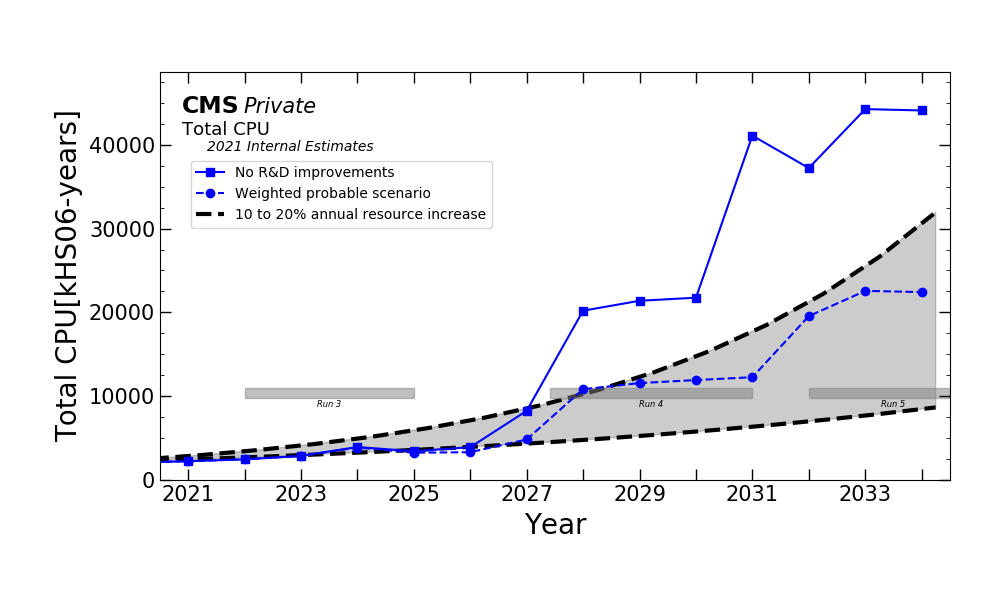
\includegraphics[trim={1.3cm 1.5cm -.5cm 1.3cm}, clip, width=.85\textwidth]{Figures/CPU_proj.png}
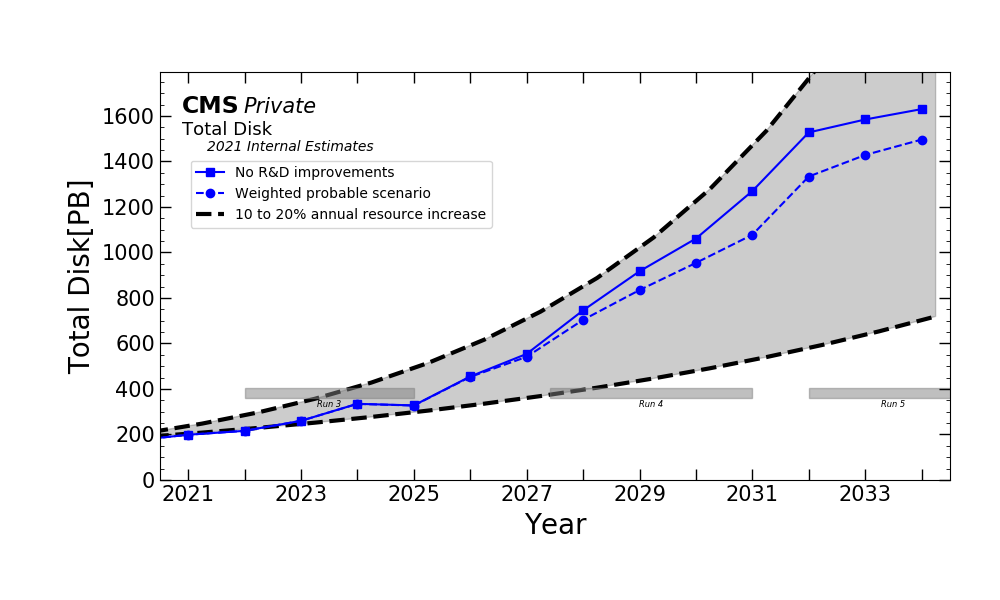
\includegraphics[trim={1.3cm 1.5cm -.5cm 1.3cm}, clip, width=.85\textwidth]{Figures/Disk_proj.png}
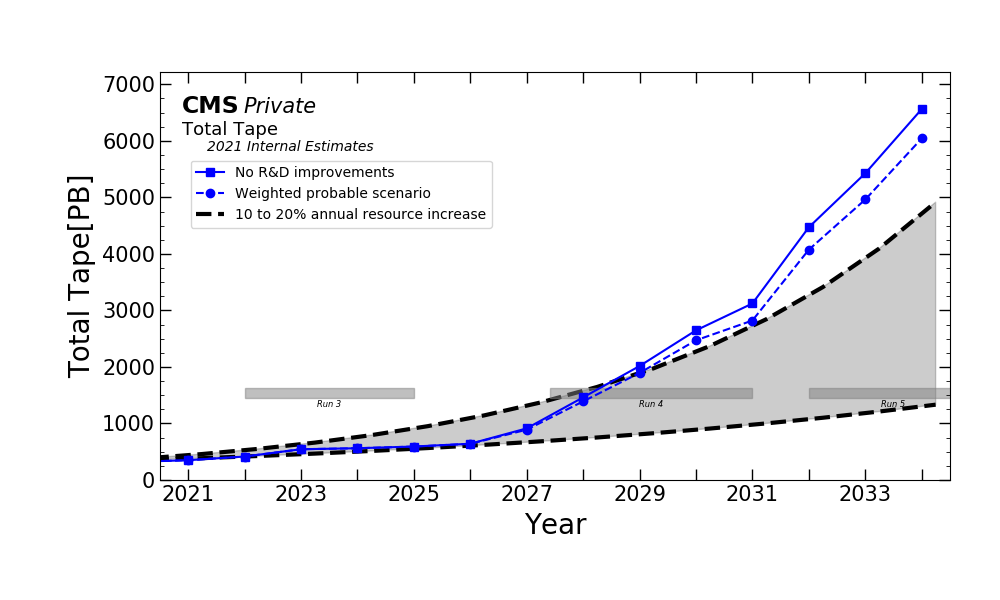
\includegraphics[trim={1.3cm 1.5cm -.5cm 1.3cm}, clip, width=.85\textwidth]{Figures/Tape_proj.png}
\caption{Projections of needed CPU, disk and tape needs into HL-LHC. On each plot a gray band represents the projected capacity of the resource within flat budget. Two lines are drawn, each corresponding to one of the two scenarios considered (\textit{Baseline} and \textit{Weighted Probable}). The latter incorporates the improvements summarized in Table~\ref{tab:two_scenarios_params}. The effect of GPUs is not represented in these plots. The tape projected needs increases almost linearly driven by the RAW data stored.}
\label{fig:projections}
\end{figure}
%
\newpage
%
\begin{figure}[ht]
\centering
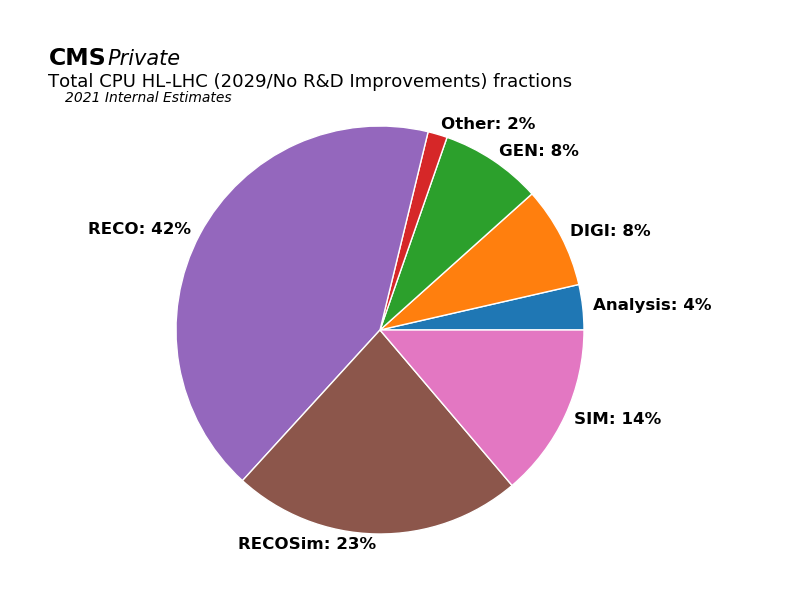
\includegraphics[trim={0cm 1.2cm 1cm 0cm}, clip, width=.4\textwidth]{Figures/CPU_pie.png}
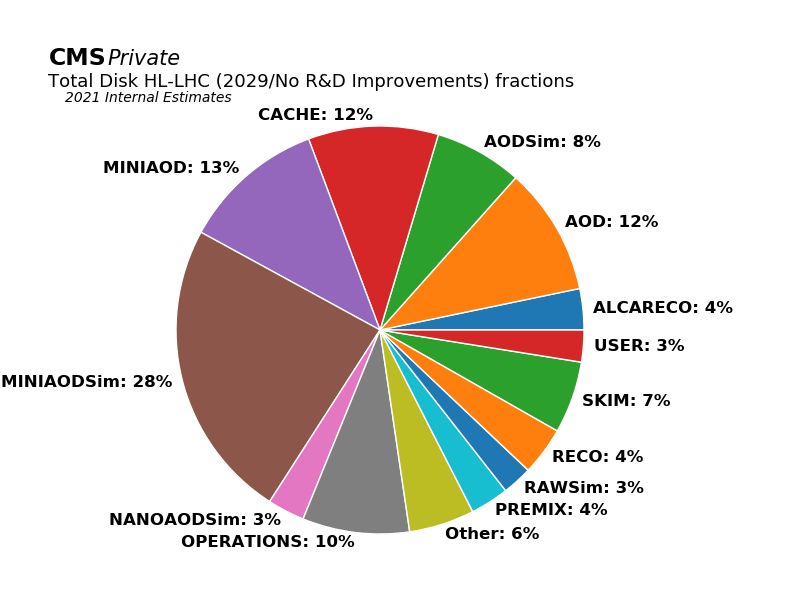
\includegraphics[trim={ 0cm 1.2cm 1cm 0cm}, clip, width=.4\textwidth]{Figures/Disk_pie.png}
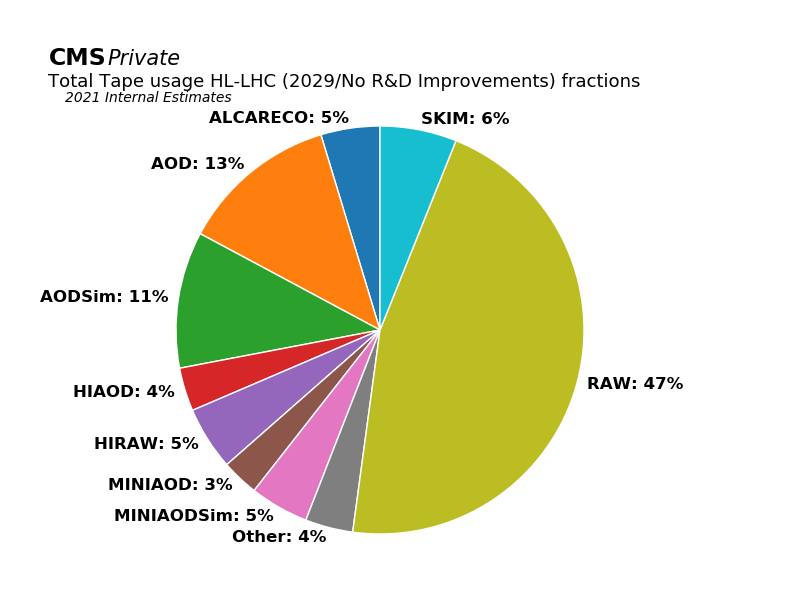
\includegraphics[trim={0cm 1.2cm 1cm 0cm}, clip, width=.4\textwidth]{Figures/Tape_pie.png}
\caption{Breakdown of the usage of CPU, disk and tape in 2030 for the Baseline scenario. Reconstruction is still the top consumer of CPU, tape usage is driven by RAW data, while most disk is used for Monte Carlo simulations.}
\label{fig:piecharts}
\end{figure}

The usage of GPUs does not lower the absolute need of computing power, but rather opens up new opportunities to CMS. In order to estimate the impact of the availability of GPUs in our infrastructure, we illustrate how the effective compute resource capacity increases if 20\% of the simulation and 25\% of the reconstruction compute is GPU instead of CPU (see table~\ref{tab:summary-gpus}), as shown in Figure~\ref{fig:gpu_impact}. 
We assume the same purchasing power implied by the 10\% to 20\% annual resource increase and that CMS can perform the aforementioned percentages of offline work on GPUs starting in 2025. 
For the purpose of deriving the annual purchase of compute needed to achieve the 10\% to 20\% resource growth, we assume that compute resources are retired in 8 years. From this, the ratio of HS06 per unit cost (2.8, see table~\ref{tab:scenarios}), and the total usable GPU fraction are used to derive the available HS06 including the GPU resource. These very conservative assumptions result at the end of Run 4 in an increase of compute capacity quantified between 20\% and 26\% for a 20\% and 10\% annual resource increase respectively.

\begin{figure}[ht]
\centering
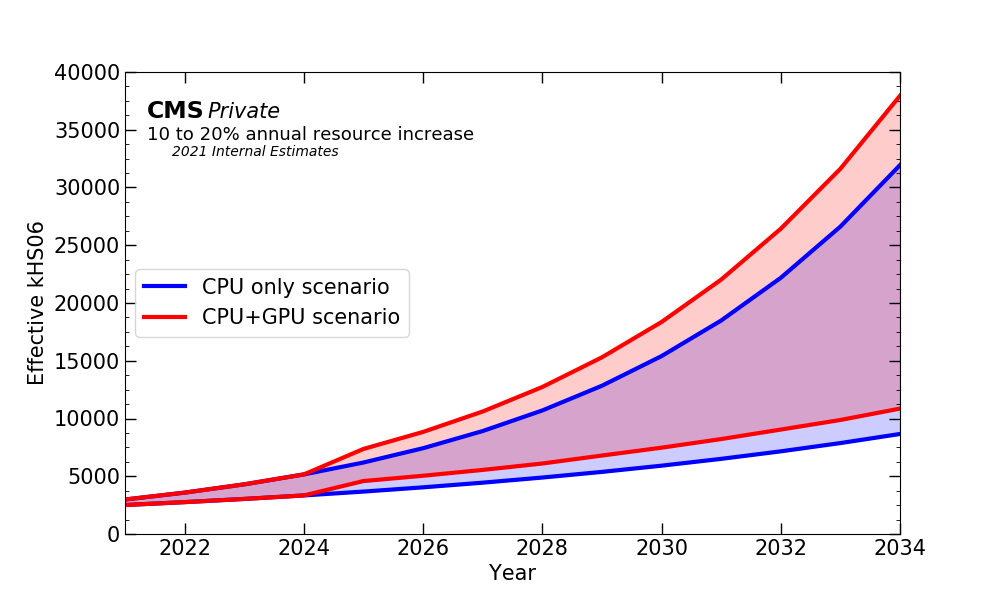
\includegraphics[trim={.5cm .5cm 1cm 1cm},clip=true,width=.55\textwidth]{gpuimpact.png}
\caption{Impact of GPUs on the compute capacity available for the same cost. The two bands illustrate the increase in available compute resources, in units of HS06, if 20\% of the simulation and 25\% of the reconstruction compute offline can be expressed through GPUs starting in 2025.
The upper (lower) limit of the band corresponds to an annual purchasing power corresponding to a 20\% (10\%) annual increase in CPU availability as was WLCG guidance for resource evolution. The GPU curve assumes the same spending profile but with additional purchasing power due to the lower cost per HS06 of GPUs.}
\label{fig:gpu_impact}
\end{figure}

%%%%%%%%%%%%%%%%%%%%%%%%%%%%%%%%%%%%%%%%%%%
\section{Summary and Conclusions}
\label{sec:conlusions}
The overall strategic goals of the CMS Offline Software and Computing coordination area are (1) to minimize the computing resource needs of the experiment and (2) to efficiently use all of the computing resources available to the experiment while maximizing throughput, all while (3) minimizing human effort in operations and software development. In this document we have described aspects of the plans CMS has to face the challenge that the HL-LHC will pose, focusing on reducing compute and storage requirements as well as enabling the utilization of hardware accelerators and HPCs, resources that the experiment must learn to use efficiently and seamlessly.

The computing resource needs are partly driven by the estimates of the operating conditions of the accelerator, communicated by the LHC machine experts, and adopted identically by CMS and ATLAS. There is a steep dependency of computing needs on the number of simultaneous collisions per bunch crossing (pileup). A distinction has been made between Run 4 with a maximum pileup of 140 and Run 5 with an ultimate pileup of 200. The most optimistic performance projections from the LHC state that a pileup of 200 could be reached in 2033 at the earliest, i.e. in twelve years at the time of writing. However, we look at that level of pileup as the ultimate challenge to be addressed by our software and computing tools, mitigating the risks that the machine out-performs expectations or software development effort becomes scarce in the second half of the 2020's.
Additionally, in agreement with WLCG, an assumption of a yearly increase of capacity for disk, tape, and CPU equivalent to 15$\pm$5\% starting from the baseline of the pledges in 2018 was adopted by CMS. This estimate takes into account cost evolution in a flat-funding scenario as well as the replacement of retired equipment. In order to reflect the impact of the usage of accelerators on computing costs, we assume, in line with the CMS HLT-DAQ TDR, a working scenario which foresees the cost per unit of computation of GPUs to be 2.8 times lower than the one of CPUs. 

We described the highly flexible computing model of CMS, characterizing at a high level the data processing tasks performed on our distributed computing system. We also highlighted how such flexibility does not come at the price of overexposing CMS to network-related risks more than other experiments.

The framework in which CMS tracks progress of the ongoing set of activities aiming to evolve our computing model was also established. It features quantitative estimates of resource savings and risk mitigations, milestones, decision points and the effort needed to achieve the results.
Oversight of these efforts is provided by CMS management, while the activity coordination is performed by the individual development areas within the offline software and computing, detector, and physics organizations. Since funding is primarily provided by the various countries and institutes, coordination is done with a collaborative and cooperative spirit.
In the rare cases when decision points exclude one or another project from being adopted by the experiment, management attempts to make the choice with full transparency, considering the technological performance and sustainability of the solutions.
If it becomes necessary to prioritize R\&D projects, for example due to effort constraints, we consider early reductions of resource needs or risks for Run 3 to be more important, also considering the cost/benefit ratio weighted by the probability of success.

The strategic goal to minimize computing resource needs is furthered by R\&D lines which aim to reduce storage and CPU requirements. For storage, we have described activities such as data format size reduction, basic processing of RAW data from the tracker and further adoption of the slimmest data format, NanoAOD, for analysis. 
%Data caches are another promising avenue of research, but the impact is difficult to quantify at this time. 
For CPU needs, we have described the potential impacts of Geant4 improvements and greater adoption of the Fast Monte Carlo Chain in the simulation. Improvements to event generators are expected, but driven by external groups. Reconstruction is where historically we have made significant progress, and we expect such continuous optimization of the reconstruction code to continue at least until the start of Run 4. Optimization of p$_\mathrm{T}$ cuts for displaced tracks, mkFit and HGCAL reconstruction with TICL can all have quantifiable impacts on CPU needs for Phase-2. Partial prompt reconstruction can also be used to reduce CPU and storage needs. However, it is a drastic action that will be considered only if we are forced to cope with the failure of other approaches, that would allow us to reduce the CPU, disk and tape needs by 35\%, 10\% and 5\%, respectively.
The efforts targeting the elimination of negative weights in event generation have an impact both on storage and CPU projected needs since they allow to reduce the total number of Monte Carlo events processed for the same statistical power. These R\&D projects are occurring entirely outside of CMS in the event generator development community and seem to be progressing well.

The second strategic goal is to efficiently use all of the computing resources available to the experiment while maximizing throughput. Access to HPCs and accelerators falls under this strategic goal.
The status of the utilization of HPCs was presented. The ability of CMS of utilize HPC centers for all central data processing workflows has been growing significantly during the last three years: the average used capacity tripled in 2020 with respect to 2019, and, at the time of writing, the average used capacity in 2021 tripled with respect to the one of 2020.
%Presently, thanks to a set of integration strategies, all with no to minimal impact on the costs of computing operations, CMS is able to use stably in a steady state tens of thousands of CPU cores at HPC centers. 
Thanks to a set of integration strategies, CMS is presently able to use tens of thousands of CPU cores at HPC centers stably and in a steady state, all with no or minimal impact on the costs of computing operations.
While the usage of HPCs does not reduce \textit{per se} the computational needs of CMS, it is a strategic choice to be flexible enough to incorporate these resources in our pool given their prominent and growing presence in the landscape of scientific computation and industrial applications.

An observable trend in the computing infrastructure at our disposal is the increasing presence of heterogeneous platforms featuring hardware accelerators such as GPUs. The status of the utilization of GPUs in CMS was described. CMS will use GPUs in its HLT farm starting in 2022. The CMSSW framework, common to all CMS applications such as generation, simulation, reconstruction and the HLT, already provides the functionality to orchestrate the offload of calculations on accelerators. The CMS workload management system can schedule jobs based on the presence of a GPU. The projected reduction of costs for distributed computing is not only related to the amount of code CMS offline applications will be able to offload on GPUs, but also the cost ratio per unit computation of GPUs and CPUs. Assuming a cost ratio per unit of compute capacity between CPU and GPU of 2.8, a flat budget, and an offload to GPU of 20\% of the simulation as well as 25\% of the reconstruction work, we could profit from a 20\% to 26\% increase in available compute capacity at the end of Run 4.
However, the ability to use accelerators is an asset regardless of cost, since HPCs and other computing resources are likely to offer not only CPUs, and mitigates the risk that we will not be able to run on entire categories of resources since the policies of providers may require the efficient usage of CPUs and accelerators.

The third strategic goal is to minimize manual operations and effort, the human side of the resource needs challenge. As an experiment ages, software development and operations effort becomes more uncertain, so efficiency in this area is no less important than minimizing hardware resource needs or integrating HPCs and accelerators into the computing infrastructure, as mentioned in section~\ref{sec:scalabilityWM}.

% Strategy Forward, with timelines
The most promising activities have been described that reduce the gap between projected availability and needs of resources or mitigate risks. The activities which have today a quantifiable reduction effect on the gap between projected availability and needs or are judged to mitigate an identified risk have been described. Their timelines, impacts, person power needs, probability of adoption as well as their associated risks have been quantified and characterized. Moreover, specific dependencies on external software packages have been discussed. We also underlined that, even if, as as an experiment ages, effort to produce innovative advancements generally declines, from time to time new ideas arise which may have additional, unforeseen impacts.

Finally, the projected resource needs have been assessed for two different scenarios for Run 4 and Run 5. The first scenario is called \textit{Baseline} and is the extrapolation of the current computing model, practices and software performance to the HL-LHC era. The second one, called \textit{Weighted Probable} scenario, is the scenario of the weighted probable outcome of the R\&D activities we considered.
At the end of Run 4, when considering the \textit{Weighted Probable} scenario, the projections of needed disk and CPU resources are in line with the available capacity. For what concerns tape, projected needs are still above the projected capacity by 20\% at the end of Run 5 and driven by the number of RAW events recorded and their sizes. Projections are affected by uncertainties, especially the ones affected by market trends of computer hardware: getting nearer to the lower part of the availability band does not necessarily mean solving the HL-LHC computation challenge. 

The \textit{Weighted Probable} scenario represents a possible solution for the HL-LHC computing challenge and already shows great promise, even only considering R\&D efforts which have today, six years before the planned start of Run 4, a quantifiable impact on computing resources needs or mitigation of identified risks. Our flexible approach and solid framework will allow us to track progress of the most mature R\&D activities and to incorporate the nascent ones. 

%%%%%%%%%%%%%%%%%%%%%%%%%%%%%%%%%%%%%%%%%%%
\newpage
\appendix
\section{Common software activities: requirements, timelines, contributions}
% %
% % Outline of high-level requirements, expected timelines, and any contributions they intended to make to the Common Software Activities.Please note dependencies and any special functionality, external packages, or interfaces required.
% %
In the charge for the review of common software activities, we were asked to outline high-level requirements, expected timelines, and any contributions that the experiment intended to make to those common software activities, noting any external dependencies or interfaces required. %Contributions in the context of the review is understood mean effort that is coordinated centrally by the experiment.

The high-level requirements in the areas of simulation, ROOT foundation, analysis, DOMA tools, and event generators, outlined in the subsections that follow, were communicated either in dedicated mini-workshops that took place in the second quarter of 2021 in the case of simulation, analysis, and DOMA, or through pre-existing regular channels of communication with the development communities.

The CMS Offline Software and Computing coordination area does not maintain a budget for software development effort, only for maintenance and operations (M\&O). However, in each of the areas covered by the review, CMS members are active participants in the respective development communities. Estimations of current and future levels of such contributions of effort are also listed.

\subsection{Simulation}
Communication and discussion of the following high-level requirements for simulation took place in a dedicated mini-workshop held on April 29, 2021~\footnote{\url{https://indico.cern.ch/event/1028379/}}.
The summary of the high level requirements for the start of Run 4 is the following:
\begin{itemize}
    \item Keep up the yearly software performance improvements or increase them. The aspirational objective of halving the time per event simulated seems adequate.
    \item Continue to provide options to tune software performance such as VecGeom~\cite{Wenzel:2754098} and improved physics lists to the needs of CMS. Moreover, adequate interfaces should be preserved and further enhanced to plug into Geant4 CMS specific simulation methods such as parametrized forward showers.
    \item Preserve or improve the physics accuracy improvements of Geant4, aiming for high quality simulation of response of new sub-detectors in CMS, most notably HGCAL.
    \item CMS is interested in testing any new GPU targeted prototype of Geant4. Working beta versions should be provided to CMS as they become available.
    \item CMS is interested in common ML driven solutions for simulation provided. Innovations in this direction should be provided to CMS as soon as they become available.
    \item At least one person from the core Geant4 team needs to be actively engaged with the simulation activities in CMS, notably for the integration of new versions or tuning of new models.
\end{itemize}

Estimated contribution of effort by CMS members to  development activities for common software in the area of simulation is 1.7 FTE to Geant4 in the form of four persons with different levels of commitment dedicated to the areas physics, geometry and validation. There are no current contributions of effort to DD4Hep, as we CMS are effectively a user. However, in 2020 there was some level of contribution stemming from the CMS integration effort.

\subsection{ROOT Foundation}
Communication and discussion of the high-level requirements for the ROOT Foundation took place in the context of regular channels of communication with the ROOT development team in the context of the ``ROOT and Experiments'' meeting~\footnote{\url{https://indico.cern.ch/category/11833/}} and private communication. 
The summary of the high level requirements for the start of Run 4 is the following:
\begin{itemize}
    \item Continue the work on ways to efficiently represent the CMS data model in the ROOT file format, delivering a slimmer and more efficient version of the ROOT columnar storage, also allowing to reduce the storage needs.
    \item Preserve and improve the thread friendliness of the ROOT core type system and IO layer, therewith allowing good scaling with the number of cores of CMS applications writing and reading from storage.
    \item Continue to support web-based graphics, expanding its functionality, most notably in the area of event visualization.
    \item Keep the ROOT core up to date with respect to the evolution of external software technologies, most notably newer C++ standards or integration with Python.
\end{itemize}

The estimated contribution of effort by CMS members to development activities for Foundation components of ROOT is at the level of 1.2 FTEs and is focussed on I/O, just-in-time compilation, automatic differentiation and data compression.
%This contribution is divided in 0.5 for I/O, 0.5 JIT/automatic differentiation, 0.2 for targeted R\&D efforts such as compression algorithms. % Too precise wrt the others
On top of these more structured commitments, punctual development activities take place in CMS which then materialize as code contributions to the ROOT repository, often coming from the Core Software area.

%From Tulika (US CMS Ops Program contribution): 0.55 FTE of Philippe Canal and 0.25 FTE of Vasile Vassilev, so a total of 0.8 FTE. Need to verify other contributions.
% Then .25 from David

\subsection{Analysis tools}
Communication and discussion of the following high-level requirements for analysis took place in a dedicated mini-workshop held on May 4, 2021~\footnote{\url{https://indico.cern.ch/event/1028381/}}.
The summary of the high level requirements for the start of Run 4 is the following:
\begin{itemize}
    \item Efficiency of analysis is of primary importance. The analysis of data must be as fast as possible, to allow physicists to have a fast turn around and try new ideas. 
    \item Fitting strategies should evolve. Methods based on finite differences should be improved to cope with the increase of the data to analyze. In particular considering the growing interest for unbinned fits.
    \item Flexibility in the access of storage is key. The highest read rate possible should be achieved when reading remotely (e.g. through XrootD remote reads), accessing local mass storage (e.g. EOS), utilizing data caches (e.g. XCache) or local fast disks.
    \item Communication and collaboration between teams providing analysis packages is a fundamental aspect of the success of the future CMS analysis: it should be preserved and enhanced.
    \item Interoperability between the products provided by different teams has to be guaranteed, minimizing data conversion. Collaboration between different library providers is also to be pursued.
    \item Ergonomic user interfaces to powerful underlying libraries must be offered to analyzers, aiming to minimize boiler plate code and potential mistakes.
    \item Active engagement is needed by the development team of analysis libraries with the analysis activities in CMS, to adapt new versions of the tools to analysis and other use cases of the experiment (e.g. alignment, calibrations).
\end{itemize}

The estimated contribution of effort by CMS members to development activities for common software in the area of analysis tools is 3-4 FTEs focusing on Python ecosystems and analysis facilities R\&D.

% From Oli
% Ops: 0.75 FTE in python ecosystem R&D: Pivarski and Ianna
% Ops: 1.10 FTE in analysis facility R&D (FNAL and various other institutes)
% There are a lot of contributions from the research budget which are hard to quantify:
% Lindsey, Nick, Matteo, other university groups are investing into coffea like approaches
% There is also IRIS-HEP, and direct shared investment are a lot, I don’t know all their fractions
% Pivarski 0.75, Ianna 0.5, but there are also Oksana and other who are paid and working on this

\subsection{DOMA tools}
Communication and discussion of the following high-level requirements for DOMA tools took place during two mini-workshops held on June 1, 2021 for RUCIO, FTS, and networking~\footnote{\url{https://indico.cern.ch/event/1043829/}} and on June 8, 2021 for storage technologies~\footnote{\tt{https://indico.cern.ch/event/1043848/}}.
The summary of the high level requirements for the start of Run 4 is the following:
\begin{itemize}
    \item Incorporate strategies for packet marking, traffic shaping and SDNs into FTS/RUCIO in a way which is transparent to CMS.
    \item Support for large ($>$100 GB) file transfers to ease Tier-0 operations in the HL-LHC era, also easing the burden on bookkeeping tools. 
    \item The stability and scalability of xRootD is very important as well as its reliable monitoring. A mechanism to throttle traffic for categories of users, for example at a certain site, is very desirable.
    \item CMS requires excellent performance for all the storage technologies (e.g. Echo, dCache, EOS), including support for streaming data from storage elements and support for (partial) reads of columnar datasets.
    \item XCache support is needed in the HL-LHC era.
    \item Four of the seven CMS Tier-1 sites (RAL, Fermilab, JINR, and PIC) are either installing, evaluating, or interested in evaluating CTA as a common software solution for tape management. CERN support for a ``CTA users community'' for use at Tier-1 sites would be highly desirable.
    \item While we appreciate the current open and transparent open source model behind RUCIO and are very happy with the collaboration with RUCIO developers, we note an asymmetry with respect to other common software projects in HEP, that none has its core development team inside a particular experiment. Even if not a problem today, unforeseen issues affecting sustainability could arise in the next 5 years, such as changes of research direction or priorities of the team where RUCIO is mainly developed or effort cuts. Complementing the current RUCIO development effort with experiment-independent supporting contributions would mitigate these risks.
\end{itemize}

There are currently no significant contributions of effort by CMS members to development activities for common software in the area of DOMA tools such as RUCIO, apart from CMS-specific tasks, although there have been contributions in the past, e.g. the Kubernetes set-up. There is a recognized need to contribute to RUCIO development which may not immediately benefit CMS at the level of 2 FTE. Examples of tasks CMS could contribute to if we had effort include token authorization, Globus Online Transfers and a generic dynamic data management daemon that could be used in CMS.
% See: https://docs.google.com/document/d/1Isf0GoE725LJaI4tfNST45pQu1thUQvtXiICXbeZQR0/edit

\subsection{Event generators}
Communication and discussion of the high-level requirements for event generators took place in the context of regular channels of communication in the HSF Event Generator Working Group~\footnote{\url{https://indico.cern.ch/category/8460/}}.
The summary of the high level requirements for the start of Run 4 is the following:
\begin{itemize}
    \item The Monte Carlo generators community should make software performance a priority, investing effort in reducing the time per event as well as the overall memory footprint needed today.
    \item Negative weights can have a substantial impact on the CPU and storage resources needed for the creation of simulated datasets. The event generators providers should continue the current work being done in this area, with the aim to eliminate or, at least, greatly mitigate the issue of negative weights.
    \item The worflows of CMS are multithreaded. Event generators should work well in a multithreaded environment (e.g. multiple instances of the same generator should be usable within the same process), not obliging CMS to adopt ad-hoc solutions to work around this limitation. More in general, event generators should be designed to work in a multithreaded environment on a distributed computing systems which has the objective to generate tens of billions of events per year.
    \item CMS is interested in testing any new GPU-based prototype of event generators. Working beta versions should be provided to CMS as they become available keeping into account the constraints a modern HEP data processing framework impose on the external packages it relies on. For example, the interface of the new generators should not change with respect to the one provided by the CPU based counterpart and no assumption shall be made about the characteristic of the underlying platform: the settings of the data processing framework will have to be easily propagated to the event generator.
\end{itemize}

%Estimated contribution of effort by CMS members to external development activities for event generators currently includes 0.8 FTE for co-authoring event generators, 0.2 FTE for work on tuning tools, and 0.1 FTE on other servcice tasks, for a total of 1.1 FTE. % too precise
Estimated contribution of effort by CMS members to external development activities for event generators currently includes 1.1 FTEs focussed on co-authoring event generators, tuning tools, and other servcice tasks.

\subsection{Summary of contributions}
Table~\ref{tab:cs_contributions} summarizes the effort that CMS manages dedicated to common software activities. We are aware that CMS is contributing much more to common software projects in a less organized way. For example, many CMS collaborators fully embrace the open source model that characterizes the cornerstones of our software stacks. They contribute valuable code, bug reports, pieces of documentation, or early testing even if not directly managed centrally by the Experiment.

\begin{table}[ht]
\begin{center}
\caption{Summary of the contributions centrally coordinated by CMS to common software activities.}
\label{tab:cs_contributions}
\begin{tabular}{lcl} 
\hline
\rowcolor{tableheader} \B{Activity} & \B{FTE} & \B{Areas} \\
\hline  \hline
\trh Simulation             & 1.7                   & Physics, geometry, validation \\ 
\trh ROOT Foundation        & 1.2                   & I/O, JIT, automatic differentiation, event display, compression \\ 
\trh Analysis Tools         & 3-4                   & Python ecosystems and analysis facilities R\&D\\ 
\trh DOMA Tools             & $-$                   & If effort were available, token authorization, Globus \\
\trh                        &                       & Online transfers, generic dynamic data management daemon \\
\trh Generators             & 1.1                   & Co-authoring, tuning tools, service tasks \\
\hline
\end{tabular}
\end{center}
\end{table}

%%%%%%%%%%%%%%%%%%%%%%%%%%%%%%%%%%%%%%%%%%%%%%%%%%%%%%%%%%%%%%%%%%%%%%%%%%%%%%%%%%
\newpage
\section{Answers to recommendations received in July 2020}
In the following, we schematically summarize the recommendations and suggestions received by the Review Panel in July 2020 and accompany them by our answers and references in the text of this document.

\subsection{Recommendations specific to CMS}
\B{Recommendation-1: Parking data was outlined as a possible mechanism to enable CMS to balance the overall cost of resources needed at the Tier-0. The documents were inconsistent on how and when data parking would be used and we encourage CMS to clarify this point.}

We addressed the topic of \textit{partial prompt reconstruction} in this section~\ref{sec:partial_prompt}.

\B{Recommendation-2: CMS noted concerns about the future of Cold Storage (Tape) and the need for R\&D on how to best use Fast Storage. However, no related plans were presented. We encourage CMS to formulate a plan.}

All LHC experiments rely on tape as archival storage. The future of tape has been discussed with WLCG and other experiments: we believe that an effective strategy to cope with a potential disappearance or prohibitive cost of this medium can only be formed within WLCG~\cite{Ahn_HSF}. More information can be found in the DOMA document prepared for this review. The status and plan of the fast storage usage has been discussed in section~\ref{subsec:fast_storage} of this document.

\subsection{Recommendations common to CMS and ATLAS}
% These are not explicit common recommendations but things underlined in the feedback that sound as recommendations. For our information.
% \B{It was not uniformly clear how much of the expected future improvements, if any, were included in the modeling.}

% We made sure this aspect is clarified in section~\ref{sec:lines_which_reduce}. Projections are presented and discussed in section~\ref{sec:projections}.

% \B{The reviewers felt that whilst ATLAS and CMS discussed a number of ways future requirements could be reduced, this stopped short of presenting a roadmap for the next few years.}

% We tried to make our roadmap as clear as possible in the text, summarizing it in section~\ref{sec:plan_for_the_evo} in a schematic way. Figure~\ref{fig:gannt} shows the timeline of this roadmap.

% \B{Many of the potential gains depend (partly or entirely) on projects external and/or collaborative projects (eg DOMA and Event Generator/Detector Simulation improvements). In some of these cases, there is a responsibility for ATLAS and CMS to provide input/requirements; to deploy and test; and to possibly adapt the computing model to incorporate. However, in all these areas, ATLAS and CMS will need to understand the expected benefits, current status, and level of risk contributed to their overall strategy.}

% We support this comment and addressed it in the text of section~\ref{sec:storage_needs} for ROOT, in section~\ref{subsec:cpu_needs_sim} for Geant4 and in section~\ref{subsec:cpu_needs_gen} for event generators.

% \B{ATLAS and CMS should examine whether their future computing model overly exposes them to a risk from networking compared to other experiments.}
% This recommendation is addressed in section~\ref{sec:risks_from_networking}.

\B{Recommendation-1: ATLAS, CMS need to iterate with WLCG and with the LHC Machine Group on a set (or sets?) of common and realistic parameters that are appropriate for baselining the computing models. Once agreed, these parameters should be used consistently. In addition to common machine and running parameters, these agreed parameters should include (a) an agreed expected cost evolution of resources and (b) the expected lifetime of hardware so that hardware replacement costs can be properly included.}

The machine parameters as well as the expected cost evolution of the hardware assumed in this document are agreed with WLCG and described in section~\ref{sec:scenarios}.

\B{Recommendation-2: Starting with the performance of the current software stack and existing computing model, ATLAS and CMS should produce tables showing how they expect CPU and storage requirements to be mitigated by current and future developments, within and outside of ATLAS and CMS, and assess the status and risks associated with each of these developments. These tables would then underpin a credible strategy.}

We added one such table for each of the sections about storage, CPU, GPUs and HPCs. We summarized all the information in section~\ref{sec:plan_for_the_evo}.

\B{Recommendation-3: ATLAS and CMS should develop R\&D roadmaps that are informed by strategy developed in the previous recommendation.}

The overall CMS strategy is described focusing on storage and CPU in section~\ref{sec:storage_needs} and section~\ref{sec:cpu_needs} respectively. Moreover, it is summarized in section~\ref{sec:plan_for_the_evo}.


%%%%%%%%%%%%%%%%%%%%%%%%%%%%%%%%%%%%%%%%%%%%%%%%%%%%%%%%%%%%%%%%%%%%%%%%%%%%%%%%%%
% THIS IS THE END ... 
%%%%%%%%%%%%%%%%%%%%%%%%%%%%%%%%%%%%%%%%%%%%%%%%%%%%%%%%%%%%%%%%%%%%%%%%%%%%%%%%%%

\newpage
\printbibliography
\end{document}
